\documentclass[journal]{vgtc}                % final (journal style)
%\documentclass[review,journal]{vgtc}         % review (journal style)
%\documentclass[widereview]{vgtc}             % wide-spaced review
%\documentclass[preprint,journal]{vgtc}       % preprint (journal style)
%\documentclass[electronic,journal]{vgtc}     % electronic version, journal

%% Uncomment one of the lines above depending on where your paper is
%% in the conference process. ``review'' and ``widereview'' are for review
%% submission, ``preprint'' is for pre-publication, and the final version
%% doesn't use a specific qualifier. Further, ``electronic'' includes
%% hyperreferences for more convenient online viewing.

%% Please use one of the ``review'' options in combination with the
%% assigned online id (see below) ONLY if your paper uses a double blind
%% review process. Some conferences, like IEEE Vis and InfoVis, have NOT
%% in the past.

%% Please note that the use of figures other than the optional teaser is not permitted on the first page
%% of the journal version.  Figures should begin on the second page and be
%% in CMYK or Grey scale format, otherwise, colour shifting may occur
%% during the printing process.  Papers submitted with figures other than the optional teaser on the
%% first page will be refused.

%% These three lines bring in essential packages: ``mathptmx'' for Type 1
%% typefaces, ``graphicx'' for inclusion of EPS figures. and ``times''
%% for proper handling of the times font family.

\usepackage{mathptmx}
\usepackage{graphicx}
\usepackage{times}
\usepackage{epstopdf}
\usepackage{paralist}
\usepackage[tight]{subfigure}
\usepackage[usenames, dvipsnames]{color}
\usepackage{textcomp}
\usepackage{program}
\usepackage{stfloats}
\usepackage[table]{xcolor}
\usepackage{array}
\usepackage{ragged2e}
\usepackage{float}
\usepackage{tabularx}
\usepackage{pifont}
\usepackage{booktabs}

%% We encourage the use of mathptmx for consistent usage of times font
%% throughout the proceedings. However, if you encounter conflicts
%% with other math-related packages, you may want to disable it.

%% This turns references into clickable hyperlinks.
\usepackage[bookmarks,backref=true,linkcolor=black]{hyperref} %,colorlinks
\hypersetup{
  pdfauthor = {},
  pdftitle = {},
  pdfsubject = {},
  pdfkeywords = {},
  colorlinks=true,
  linkcolor= black,
  citecolor= black,
  pageanchor=true,
  urlcolor = black,
  plainpages = false,
  linktocpage
}

\definecolor{darkGreen}{RGB}{0, 100, 0}
\definecolor{nmGreen}{RGB}{225, 255, 194}
\definecolor{nmOrange}{RGB}{254, 225, 194}
\definecolor{nmYellow}{RGB}{255, 255, 208}

\newcommand*\rot{\rotatebox{90}}
\newcommand*\OK{\ding{51}}

\newcommand*\match{\textcolor{darkGreen}{\ding{52}}}
\newcommand*\mismatch{\textcolor{red}{\ding{54}}}
\newcommand*\posmatch{\textcolor{blue}{{\bf ?}}}

\newcommand{\bstart}[1]{\vspace{1mm} \noindent{\textbf{#1:}}}

\newcommand{\bqstart}[1]{\vspace{1mm} \noindent{\textbf{#1}}}

\newcommand{\bscstart}[1]{\vspace{1mm} \noindent{\sc{\textbf{#1:}}}}

\newcommand{\tm}[1]{\textcolor{red}{#1}}
\newcommand{\mb}[1]{\textcolor{blue}{#1}}

\newcommand{\etal}{et al.}
\newcommand{\eg}{e.\ g.}
\newcommand{\ie}{i.\ e.}

%% If you are submitting a paper to a conference for review with a double
%% blind reviewing process, please replace the value ``0'' below with your
%% OnlineID. Otherwise, you may safely leave it at ``0''.
\onlineid{0}

%% declare the category of your paper, only shown in review mode
\vgtccategory{Research}

%% allow for this line if you want the electronic option to work properly
\vgtcinsertpkg

%% In preprint mode you may define your own headline.
%\preprinttext{To appear in IEEE Transactions on Visualization and Computer Graphics.}

%% Paper title.

\title{From Analyzing the Energy Performance of Building Portfolios to Guidelines for Visualizing Time-Oriented Data}

%% This is how authors are specified in the journal style

%% indicate IEEE Member or Student Member in form indicated below
\author{Matthew Brehmer, Jocelyn Ng, Kevin Tate, and Tamara Munzner,~\textit{Member, IEEE}}
\authorfooter{
%% insert punctuation at end of each item
\item
 Matthew Brehmer and Tamara Munzner are with the University of British Columbia. E-mail: \{brehmer,tmm\}@cs.ubc.ca.
\item
 Jocelyn Ng and Kevin Tate are with EnerNOC, Inc. E-mail: \{jocelyn.ng,kevin.tate\}@enernoc.com.
}

%other entries to be set up for journal
\shortauthortitle{Biv \MakeLowercase{\textit{et al.}}: From Energy Analysis to Guidelines for Visualizing Time-Oriented Data}
%\shortauthortitle{Firstauthor \MakeLowercase{\textit{et al.}}: Paper Title}

%% Abstract section.
\abstract{
The energy performance of dozens or hundreds of buildings is challenging to analyze and monitor, as current analysis tools are not scalable, or they present derived and aggregated data that is too coarse.
In partnership with an energy analysis software company, we conducted a visualization design study, beginning with a thorough work domain analysis and a characterization of data and task abstractions.
We describe generalizable visualization design choices framed in terms of \textsl{matches} and \textsl{mismatches}, choices that are transferable beyond the energy domain. 
We also present guidelines pertaining to the themes of \textsl{familiarity} and \textsl{trust}, as well as methodological considerations for visualization design projects involving corporate collaborators and their external clients.
As a result of our research, our designs were adopted by our collaborator and incorporated into the design of an energy analysis software application that will soon be deployed and used by tens of thousands of energy workers.
} % end of abstract

%% Keywords that describe your work. Will show as 'Index Terms' in journal
%% please capitalize first letter and insert punctuation after last keyword
\keywords{Design study, redesign, energy analysis, task and requirements analysis, multiple time series.}

%% ACM Computing Classification System (CCS). 
%% See <http://www.acm.org/class/1998/> for details.
%% The ``\CCScat'' command takes four arguments.

\CCScatlist{ % not used in journal version
 \CCScat{H.5.2}{Information Interfaces and Presentation (e.g. HCI)}{User interfaces}{Graphical user interfaces (GUI), Evaluation/methodology, User-centered design}
}

%% Uncomment below to include a teaser figure.
%   \teaser{
%   \centering
%   \includegraphics[width=16cm]{CypressView}
%   \caption{In the Clouds: Vancouver from Cypress Mountain.}
%   }

%% Uncomment below to disable the manuscript note
%\renewcommand{\manuscriptnotetxt}{}

%% Copyright space is enabled by default as required by guidelines.
%% It is disabled by the 'review' option or via the following command:
% \nocopyrightspace

%%%%%%%%%%%%%%%%%%%%%%%%%%%%%%%%%%%%%%%%%%%%%%%%%%%%%%%%%%%%%%%%
%%%%%%%%%%%%%%%%%%%%%% START OF THE PAPER %%%%%%%%%%%%%%%%%%%%%%
%%%%%%%%%%%%%%%%%%%%%%%%%%%%%%%%%%%%%%%%%%%%%%%%%%%%%%%%%%%%%%%%%

\begin{document}

%% The ``\maketitle'' command must be the first command after the
%% ``\begin{document}'' command. It prepares and prints the title block.

\maketitle

%% the only exception to this rule is the \firstsection command
%% \section{Introduction} %for journal use above \firstsection{..} instead

%-------------------------------------------------------------------------
%-------------------------------------------------------------------------

\section{Introduction}
\label{introduction}

%-------------------------------------------------------------------------
%-------------------------------------------------------------------------

Consider a university campus containing a hundred buildings. 
For a university operations worker looking for opportunities to conserve energy, visualization can be helpful when analyzing and monitoring the energy performance of this large {\it portfolio} of buildings. 

In this visualization design study, we collaborated with a company that develops energy analysis and reporting software for organizations such as commercial business chains, universities, and utility companies.
Our collaborator's goal was to deploy a redesigned version of {\it Energy Manager}, their energy analysis software tool; in doing so, they hoped to retain their existing clients, attract new ones, and increase engagement with their software. 
{\it Energy Manager} is actively used by over 200 individuals, some of whom use it to analyze the energy performance of dozens to hundreds of buildings.
% Thousands of energy workers had access to {\it Energy Manager}, though less than 300 were engaged and actually using the tool. 
% As a result of a result partnering with a large utility company, the number of potential users will increase to potentially hundreds of thousands of individuals.
Our goal as researchers was to convince our collaborators to commit software development resources and adopt our visualization designs, designs motivated by our extensive user research.

Visualization researchers and practitioners working in non-energy-related domains will find several transferable aspects of this paper, beginning with our characterization of data and task abstractions.
In addition, this project required that we design visualizations for ``bar and line chart crowd'': we needed to promote sophisticated visual analysis by individuals accustomed to unsophisticated visual idioms.
We designed and evaluated potential visualizations with a variety of stakeholders in a corporate non-research setting, which included employees of our collaborator, as well as their external clients.
This paper also presents a {\it success story}, in which our collaborator adopted some of our visualization designs, and we make a point to document our methodology that led to this success.

\bstart{Contributions} our primary contribution is a set of generalizable visualization design choices and guidelines framed in terms of {\bf matches} and {\bf mismatches} between abstractions and techniques~\cite{Meyer2013}, guidelines that transfer beyond the energy domain.
We also present guidelines relating to the themes of {\bf familiarity} and {\bf trust}; the former refers to the spectrum between ubiquitous visual encodings and those that a prospective user may have never seen before, while the latter refers to the appropriate display of derived and aggregated data, as well as giving users control over these data transformations.
Finally, we contribute {\bf methodological advice} for visualization design projects in an industry context, where prospective users include both the collaborator's employees and their remote external clients.

\bstart{Outline} we begin by providing some background context with regards to the energy domain.
We then characterize the data and tasks in Section~\ref{abstractions}; we consider how the three tasks we characterized are supported by the existing {\it Energy Manager} tool in Section~\ref{existing-tool}, and how previous work addresses similar data and tasks in Section~\ref{related-work}.
In Section~\ref{design}, we present our designs and characterize them in terms of matches and mismatches according the three tasks.
The result of our design process, the adoption of our visualization designs into our collaborator's product development cycle, are described in Section~\ref{production}.
In Section~\ref{discussion}, we reflect on familiarity, trust, and on methodological considerations for visualization design studies in industry contexts.
Section~\ref{conclusion} summarizes our contributions.

%-------------------------------------------------------------------------
%-------------------------------------------------------------------------

\section{Domain Background}
\label{domain}

%-------------------------------------------------------------------------
%-------------------------------------------------------------------------

Prior to characterizing our data and task abstractions, we introduce the {\it energy worker}, along with their domain goals and activities.
Here we focus on findings from our work domain analysis; we comment on our methodological approach to this phase of the project in Section~\ref{discussion-methodology}. 

In the summer and fall of 2013, we conducted 9 in-depth interviews with current users of {\it Energy Manager}, our collaborator's software.
Eight of those interviewed were employed by clients of our collaborator, which included three North American universities, an engineering consulting firm, and a school board. 
The final interviewee was an employee of our collaborator who regularly consulted with new clients.  
Although we use the term {\it energy worker} to describe these individuals, we encountered a wide range of roles, job titles, skill sets, and levels of training. 
The use of energy analysis tools such as {\it Energy Manager} also varied in terms of context and frequency of use.
Despite these differences, we did identify several common goals and activities.

\bstart{Domain goals and activities} the energy workers to whom we spoke oversee the energy performance of dozens to hundreds of buildings, which are referred to as {\it portfolios}. 
They need to balance a need to reduce costs and conserve energy while ensuring the comfort and safety of people who use these buildings.
To achieve these goals, the energy workers need to: ({\bf 1}) assess the performance of buildings in their portfolio following the implementation of an energy conservation measure, such as installing new windows or lighting; ({\bf 2}) determine which buildings in their portfolio require energy conservation measures; and ({\bf 3}) find and diagnose anomalous energy performance such as spikes, outages, surges, or otherwise erratic and inconsistent behaviour.

%-------------------------------------------------------------------------
%-------------------------------------------------------------------------

\section{Abstractions}
\label{abstractions}

%-------------------------------------------------------------------------
%-------------------------------------------------------------------------

We now characterize these domain activities in terms of data and task abstractions.

%-------------------------------------------------------------------------

\subsection{Data Abstraction}
\label{data-abstractions}

%-------------------------------------------------------------------------

We begin by abstracting a portfolio of buildings and its associated time-oriented energy data, which we summarize in Table~\ref{tab:data-abstractions}.

\begin{table}[ht]\renewcommand{\arraystretch}{1.2}\addtolength{\tabcolsep}{-1pt}
    \vspace{-.3cm}
    \begin{center}
    \scriptsize
    \begin{tabular}{l|l|l}

        \rowcolor{red!15}
    
        {\bf Term} & {\bf Abstraction} & {\bf Example}
    
        \\
        
        \hline
        
        \multicolumn{3}{c} {\it Building metadata} 
        
        \\
    
        \hline
        
        Building ID & unique categorical & \#123
    
        \\
        
        \rowcolor{gray!15}
        
        Building area & quantitative & 450 m$^{2}$
    
        \\
        
        Building age & quantitative & 20 years
    
        \\
        
        \rowcolor{gray!15}
        
        No. occupants & quantitative & 50 people
    
        \\
        
        Location & spatial & 49.25$^{\circ}$ N, 123.10$^{\circ}$ W
    
        \\
        
        \rowcolor{gray!15}  
        
        Tag & categorical & {\it ``restaurant''}
    
        \\
        
        \hline
        
        \multicolumn{3}{c} {\it Temporal data for each building} 
        
        \\
    
        \hline
        
        Energy demand & quantitative & 200 kW
    
        \\
        
        \rowcolor{gray!15}
        
        Outdoor temperature & quantitative & 18$^{\circ}$ C
    
        \\
        
        Open / closed & categorical & Open Mon--Fri, 08-18h
    
        \\
        
        \hline
        
        \multicolumn{3}{c} {\it Derived temporal data for each building} 
        
        \\
    
        \hline
        
        Consumption & quantitative & 800 kWh
    
        \\
        
        \rowcolor{gray!15}
        
        Energy intensity & normalized quantitative & 1.78 kWh / m$^{2}$
    
        \\
    
        Weather-independent & normalized quantitative & ({\it P2C2E})$^\ddagger$
    
        \\ 
        
        performance$^\dagger$ & & 
        
        \\
        
        \rowcolor{gray!15}
        
        Predicted perform.$^\dagger$ & quantitative & 190 kW
        
        \\
        
        \% Savings & normalized quantitative & 40\%
        
        \\
        
        Rank & ordinal & 1st, 2nd, 3rd
        
        \\
        
        \hline  
        
    \end{tabular}
    \vspace{-0.3cm}
    \caption{Our data abstractions. $^\dagger$\textsl{Performance} could be assessed in terms of \textsl{demand}, \textsl{consumption}, or \textsl{intensity}. $^\ddagger$There are several approaches to normalizing energy performance based on weather data, though this is beyond the scope of our current discussion.}
    \label{tab:data-abstractions}
    \end{center}
    \vspace{-0.6cm}
\end{table}

\bstart{Building metadata} consider a university, where buildings vary by area, age, and number of occupants. 
Buildings can be differentiated using any number of categorical {\it tags}, such as the type of building ({\it ``lecture hall''}, {\it ``laboratory''}), its campus or department ({\it ``chemistry''}, {\it ``physics''}), or the name of its building operations manager.   

\bstart{Building groups} given all of this building metadata, we can have groups of buildings with shared attribute values or ranges. 
A portfolio may have many alternative groups, and they may overlap.

\bstart{Multiple time series per building} the energy performance of each building in a portfolio is monitored over time, and each building has multiple time series associated with it.
A building may consume several forms of energy, such as electricity, natural gas, or steam; many non-residential buildings are equipped to report raw energy demand values every 15 minutes, along with outdoor air temperature. 
Building opening and closing hours are also recorded.

\bstart{Derived data} raw continuous energy demand data is typically examined during detailed investigations of single buildings at fine granularities of time; for instance, a building might exhibit an unexpected spike in demand on a Sunday morning. 
For an energy worker overseeing a large portfolio of buildings, analysis activities typically revolve around {\it derived} and {\it aggregated} data, rather than raw continuous data. 
These include {\it averages}, {\it minimums}, and {\it maximums} for different temporal granularities of interest, such as the average weekday electricity demand in January.
{\it Consumption} is the most common of these derived attributes, which is an accumulated amount of energy.
{\it Intensity} is consumption normalized by a building's area, which allows the energy worker to directly compare the energy performance of buildings of different size.
Similarly, it is possible to normalize energy performance values by considering outdoor temperature, which allows the energy worker to compare buildings at different times of the year, or buildings in locations with different climates.
{\it Predicted energy performance} based on statistical models are also considered, though these predicted values are problematic for reasons we describe in Section~\ref{existing-tool}.
{\it Relative} and {\it absolute differences} between the observed energy performance and the predicted or historical performance are also considered; for example, the energy worker can determine how much better or worse a building is performing this year relative to its performance last year.
Finally, given any of these derived values, the energy worker can create a {\it ranking} of buildings, allowing them to identify, for instance, the 5 worst-performing buildings a portfolio.

In summary, we have a multidimensional table of buildings and building attributes, along with quantitative energy-related attributes with values changing over time.

%-------------------------------------------------------------------------

\subsection{Task Abstractions}
\label{task-abstractions}

%-------------------------------------------------------------------------

\begin{table*}[ht]\renewcommand{\arraystretch}{1.2}\addtolength{\tabcolsep}{-1pt}
    % \vspace{-.3cm}
    \begin{center}
    \scriptsize
    \begin{tabular}{p{0.125\textwidth}|>{\RaggedRight}p{0.15\textwidth}|>{\RaggedRight}p{0.15\textwidth}|>{\RaggedRight}p{0.15\textwidth}|>{\RaggedRight}p{0.15\textwidth}|>{\RaggedRight}p{0.15\textwidth}}

        \rowcolor{nmYellow}
    
        {\bf Task} & \cellcolor{nmOrange} {\bf Domain activities} & \cellcolor{nmOrange} {\bf Scope} & {\bf Abstraction: {\tt Actions}} & {\bf Abstraction: {\tt Targets}} & {\bf Concrete example}
        
        \\
        
        \hline  
        
        %task name
        \cellcolor{nmYellow} {\bf T1}: Overview 
        
        %domain activities
        & \cellcolor{nmOrange} Determine which building(s) require energy conservation measures. Find anomalous energy performance.
        
        %scope
        & \cellcolor{nmOrange} The entire portfolio of buildings, coarser time periods. 
        
        %abstraction: actions
        & {\it consume}: {\tt discover}, {\tt present}; {\it search}: {\tt lookup}; {\it query}: {\tt summarize}.
        
        %abstraction: targets
        & {\it all data}: {\tt trends}, {\tt outliers}; {\it attributes}: {\tt distributions}, {\tt extremes}, {\tt similarities}. 
        
        %example question
        & {\it ``How did my building portfolio perform this past year?''}
        
        \\
        
        \hline
        
        %task name
        \cellcolor{nmYellow} {\bf T2}: Detail 
        
        %domain activities
        & \cellcolor{nmOrange} Assess performance following energy conservation measures. Find and diagnose anomalous energy performance. 
        
        %scope
        & \cellcolor{nmOrange} A group of buildings within the portfolio, finer time periods.
        
        %abstraction: actions
        & {\it consume}: {\tt discover}; {\it search}: {\tt locate}; {\it query}: {\tt compare}. 
        
        %abstraction: targets
        & {\it all data}: {\tt trends}, {\tt outliers}, {\tt features}.
        
        %example question
        & {\it ``Are my restaurants in Vancouver performing better this January than they did last January?''}
        
        \\
        
        \hline
        
        %task name
        \cellcolor{nmYellow} {\bf T3}: Proportion 
        
        %domain activities
        & \cellcolor{nmOrange} Find and diagnose anomalous energy performance. 
        
        %scope
        & \cellcolor{nmOrange} A group of buildings within the portfolio, finer time periods. 
        
        %abstraction: actions
        & {\it consume}: {\tt discover}; {\it search}: {\tt locate}, {\tt explore}; {\it query}: {\tt identify}. 
        
        %abstraction: targets
        & {\it all data}: {\tt trends}, {\tt outliers}, {\tt features}; {\it attributes}: {\tt dependencies}. 
        
        %example question
        & {\it ``What proportion of my university's energy consumption is consumed by its computer science building over time?''}
        
        \\
        
        \hline  
        
    \end{tabular}
    \vspace{-0.3cm}
    \caption{A summary of the task abstractions (yellow) alongside their corresponding domain activities and scope (orange). The task abstractions are characterized according to a recent task typology~\cite{Brehmer2013}, distinguishing between \textsl{actions} and \textsl{targets}~\cite{Munzner2014}.}
    \label{tab:task-abstractions}
    \end{center}
    \vspace{-0.9cm}
\end{table*}

We characterize our task abstractions according to a recent task typology~\cite{Brehmer2013}, distinguishing between actions and targets~\cite{Munzner2014}. 
These three abstract tasks are summarized in Table~\ref{tab:task-abstractions}, and terms from this typology appear in a {\tt fixed-width font}.
Each of the tasks can be described by a need to {\tt discover}, to generate and verify hypotheses.
Energy workers will also occasionally {\tt present} their findings to colleagues and other stakeholders, however our current focus is preominantly on the discovery process. 

\bstart{T1 / Overview} an individual performs a {\tt lookup} and {\tt summarizes} time-oriented data from all the items spanning a coarse period of time. 
Of interest are {\tt trends}, {\tt outliers}, {\tt distributions}, {\tt extreme values}, and {\tt similarities}. 
This abstract task corresponds to the domain activities of determining which buildings in a portfolio require energy conservation measures and finding anomalous energy performance. 
A concrete example of this task would be an energy worker who asks: {\it ``how did the university perform this past year?''}.
A general question like this may also arise when {\tt presenting} findings.

\bstart{T2 / Detail} the second task is the result of drilling down from the portfolio to a group of buildings, examining energy performance in detail: an individual {\tt locates} and {\tt compares} {\tt trends}, {\tt outliers}, and {\tt features} in time-oriented data for items in the group.
This abstract task corresponds to the domain activities of assessing building performance following an energy conservation measure, or finding and diagnosing anomalous energy performance. 
A concrete example of this task is: {\it ``are my restaurants in Vancouver performing better this January than they did last January?''}.

\bstart{T3 / Proportion} the third task is the converse of drilling down from the portfolio to a group and from the group to individual buildings.
This task is one in which the individual {\tt explores} and {\tt locates} {\tt trends}, {\tt outliers}, and {\tt features} in time-oriented data to {\tt identify} the proportion of individual behaviour relative to the group's behaviour: the {\tt dependency} between the aggregate amount and the individual contribution.
A concrete example of this task is: {\it ``what proportion of a university's energy consumption is consumed by its computer science building over time?''} or {\it ``what building in the science faculty consumes the largest proportion of energy?''}.

\bstart{Task sequences} these three tasks are not performed in isolation, but in sequence, and some task sequences occur more often than others. 
We know from our interviews that the frequency of this work varies, so the Overview ({\bf T1}) task may be more prevalent among energy workers who infrequently analyze their portfolio's energy performance.
Alternatively, an energy worker may skip the Overview ({\bf T1}) task because she or he has a specific question about a group of buildings, proceeding directly to the Detail ({\bf T2}) or Proportion ({\bf T3}) tasks. 
An energy worker is also expected to {\it cycle} between the Detail ({\bf T2}) and Proportion ({\bf T1}) tasks, as the completion of one task may prompt new questions.

%-------------------------------------------------------------------------
%-------------------------------------------------------------------------

\section{Existing Tool}
\label{existing-tool}

%-------------------------------------------------------------------------
%-------------------------------------------------------------------------

Given our abstractions, we now analyze the existing {\it Energy Manager} tool and determine the extent to which the tasks are supported.

\begin{figure*}[bp!]
    \vspace{-0.6cm}
	\centering
	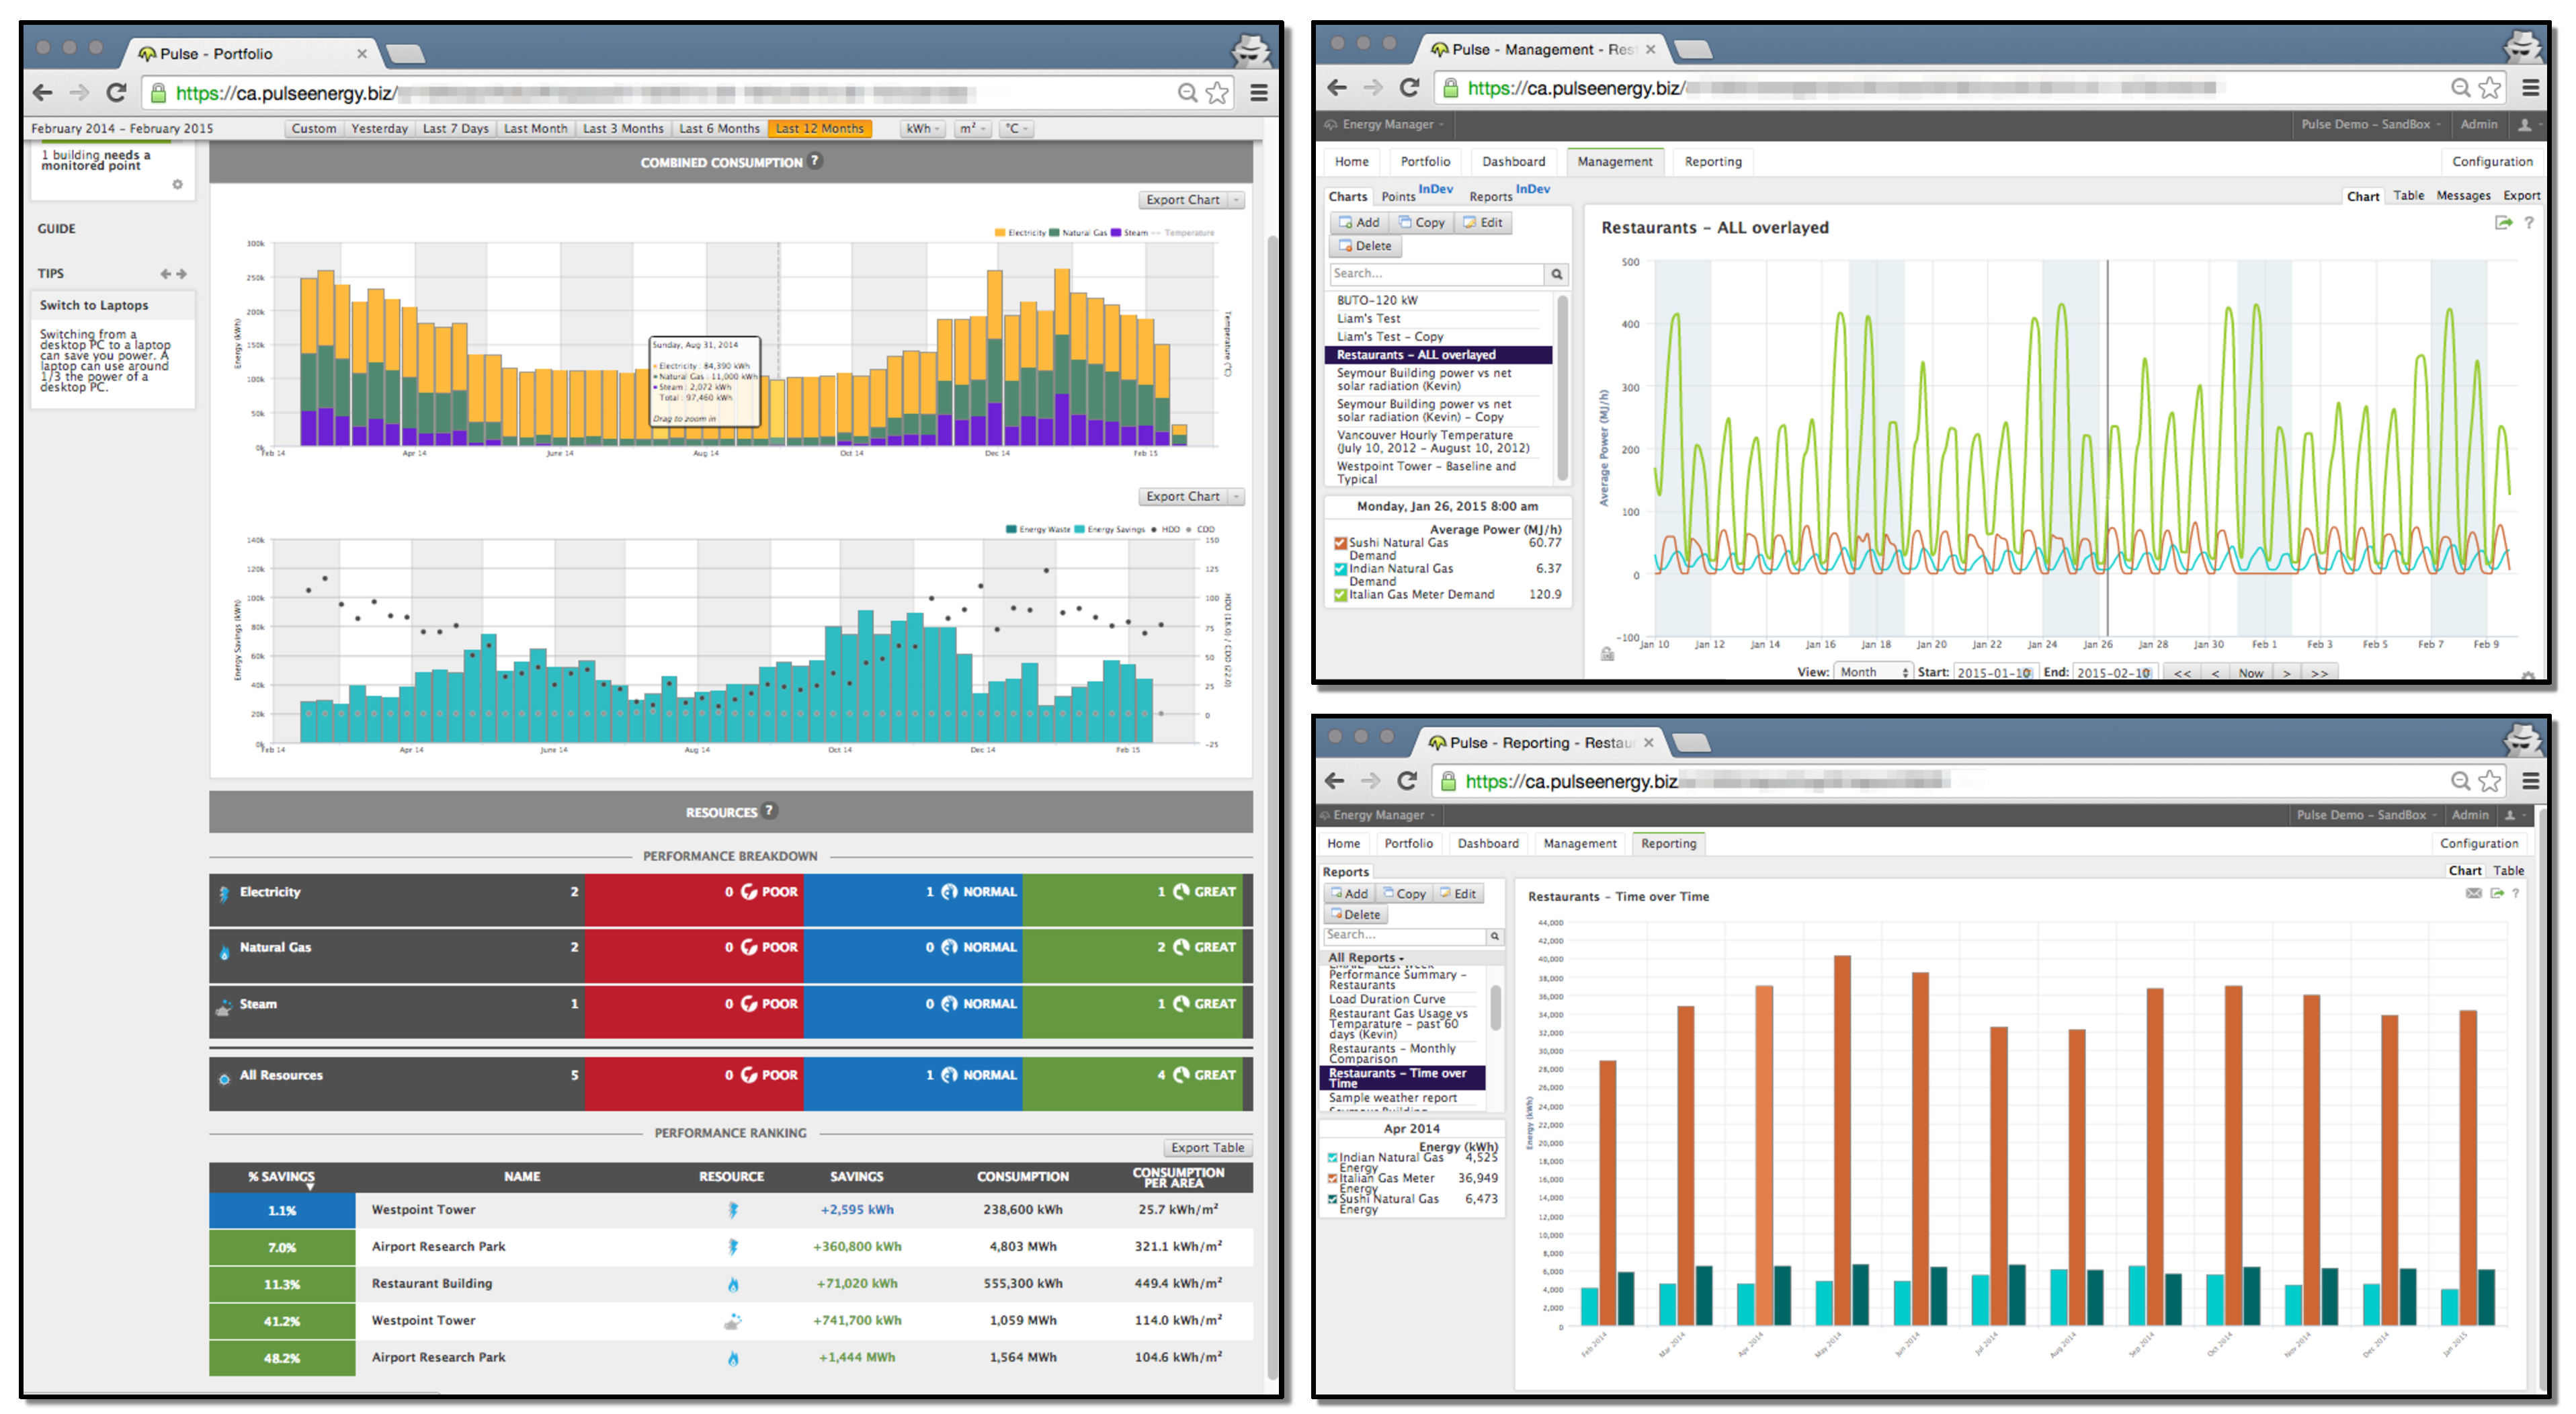
\includegraphics[width=\textwidth]{figures/em.pdf}
	\vspace{-0.6cm}
	\caption{\textsl{Energy Manager}, our collaborator's existing energy analysis tool. Left: a dashboard for a portfolio of buildings. Right: superimposed line charts of \textsl{energy demand} (top) and grouped bar charts of \textsl{energy consumption} (bottom) for a group of buildings within this portfolio.}
	\label{fig:energy-manager}
% 	\vspace{-0.6cm}
\end{figure*} 

% We focus on {\it Energy Manager} first, our collaborator's existing software, which all of the energy workers we interviewed had used to a varying extent for performing portfolio energy analysis.

{\it Energy Manager}, shown in Figure~\ref{fig:energy-manager}, is a multiple-page web-based application, one that uses a small number of visual idioms: bar charts are used for derived aggregate values such as {\it consumption}, while line charts are used for continuous values such as {\it energy demand}.
The main page presents a summary dashboard for a portfolio of buildings (Fig.~\ref{fig:energy-manager}-left). 
At the bottom of this dashboard is a sortable table listing {\it consumption}, {\it intensity}, as well as aggregate relative and absolute {\it savings} values for the currently selected time period. 

More detailed line and bar charts (e.g. Fig.~\ref{fig:energy-manager}-right) are indexed on the other pages, similar to how a Microsoft {\it Excel} workbook has sheets, which can in turn contain multiple charts. 
Unlike {\it Excel}, {\it Energy Manager}'s visualizations provide some interactivity: the user can zoom, pan, and reveal values upon mouseover. 
However, none of the visualizations are linked to one another or to the dashboard, so the energy worker must navigate between them manually.

\bstart{Task support} {\it Energy Manager} only partially supports the Overview ({\bf T1}) task: with the portfolio dashboard, the energy worker can observe the aggregate {\it consumption} for a portfolio over time, or alternatively she can observe single aggregate values for individual buildings in the sortable table, but she will not see how these individual buildings vary over time.
As a result, the energy workers that we interviewed used this dashboard sparingly, if at all, and none of them had found the sortable table to be useful.

The Detail ({\bf T2}) task is supported but the current solution does not scale, especially since superimposed line charts and grouped bar charts are limited by the number of discriminable colours.
The examples in Figure~\ref{fig:energy-manager} (right) display {\it energy demand} and {\it consumption} performance for three restaurants; what if the energy worker has thirty restaurants, or three hundred?

The Proportion ({\bf T3}) task is not explicitly supported: though it is possible to estimate the proportion of a building's energy performance relative to its group with bars and lines, this process is error-prone.

Finally, because the visualizations in {\it Energy Manager} are not coordinated or linked in any way, it is difficult and tedious to to drill down or alternate from Overview ({\bf T1}) to Detail ({\bf T2}) and Proportion ({\bf T3}) Tasks. 
As in {\it Excel}, the energy worker will have to locate an existing visualization or specify a new visualization using a wizard dialog; if the bar or line chart for a set of items does not already exist when the energy worker needs it, she has to create it. 
By the time she has created it, she may have forgotten her objective.

\bstart{Limited filtering and aggregation} the bar and line charts in {\it Energy Manager} allow an energy worker to hide or show individual buildings (notice the checkboxes in Figure~\ref{fig:energy-manager}-right).
However, the energy worker cannot filter buildings with shared attributes, such as filtering a portfolio of buildings to only show restaurants.
Similarly, it is impossible to aggregate buildings together when they share attributes: for instance, the energy worker cannot compare the aggregate energy performance of restaurants in one city to those in another.

\bstart{No faceting} aside from the seldom-used portfolio dashboard shown in Figure~\ref{fig:energy-manager} (left), there is no faceting or juxtaposition of visualizations in {\it Energy Manager}: the energy workers' workaround involved opening multiple browser windows, adjusting the line or bar charts to display the same scale and ranges, and tiling these windows manually across their monitor.

\bstart{Summary} as a result of these limitations, energy workers can only observe narrow slices of their data, or they are presented with aggregate data that is too coarse to be useful.
Similarly, they did not trust {\it Energy Manager}'s derived predicted values based on statistical models, and would have preferred to compare observed energy performance to historical performance.
In other words, the derived and aggregated values currently shown may hide information such as extreme values and unusual distributions.
As a result of this loss of detail, the energy workers that we interviewed would routinely export tabular data from {\it Energy Manager} and import it into {\it Excel}, where they would perform custom analysis or create custom reports.
Finally, we note that a survey of energy analysis software tools built by our collaborator's competitors revealed that they suffer from similar limitations, and those whom we interviewed corroborated this finding, as many of these energy workers had worked with these tools in the past.

%-------------------------------------------------------------------------
%-------------------------------------------------------------------------

\section{Related Work}
\label{related-work}

%-------------------------------------------------------------------------
%-------------------------------------------------------------------------

We now review relevant previous work, beginning with work in the energy domain. 
We also discuss visualizations of time-oriented data in other domains, as well as evaluation studies that assess the effectiveness of visualization idioms for similar data and task abstractions.

\bstart{Visualization in the energy domain} technology that allows for the continuous measurement of a building's energy demand is becoming increasingly available, and several techniques to monitor and present this data have recently been proposed, especially for residential buildings~\cite{Erickson2013,Goodwin2013,Rodgers2011}.
Erickson~\etal~\cite{Erickson2013} developed a web-based residential energy dashboard for homeowners, allowing them to compare against their neighbours with familiar bar and line charts.
However, such a dashboard would be unsuitable for the analysis work of an energy worker who oversees a portfolio of many buildings.

Though bar and line chart depictions of energy data are most common, other visual encodings have also been employed, from abstract and artistic ambient visualizations~\cite{Rodgers2011} to a compelling calendar-based visualization~\cite{vanWijk1999}, in which calendar dates with similar energy behaviour are visually associated with a common colour.
We also explore visual encodings beyond bar and line charts, including calendar-based encodings; in Section~\ref{design-matrix} we consider how to encode data from multiple buildings using calendars.

One approach to summarizing the energy behaviour of multiple buildings is to use map-based visualizations~\cite{Heat2014,MEP2014}, though these may be more appropriate for buildings in a shared neighbourhood, such as a university campus; these encodings may be less appropriate for building portfolios spanning large geographic areas.
We too explored the use of maps (see Figure~\ref{fig:sandbox}), though in speaking with energy workers we found that maps are better-suited for presenting coarse aggregate summary values of energy performance to a casual observer, and they are less appropriate for recurring analysis work; to view energy behaviour varying over time, animating or faceting the map would be necessary.
Furthermore, an energy worker overseeing a portfolio of buildings is already likely to be familiar with the locations of buildings in her portfolio, and their relative locations are not informative.
While using a map to encode energy data may not be appropriate for the tasks that we characterized, an interactive map may be an effective means to filter a portfolio by building location, and we may incorporate map-based filtering in future designs.

More closely related to our work is that of Goodwin~\etal~\cite{Goodwin2013}, who presented several prototype visualizations of modelled residential energy use across thousands of households, albeit at the scale of individual household appliances. 
The domain activities they address overlap partially with those performed by the energy workers we spoke to, such as the need to find anomalous energy performance across many buildings; another activity they address, in which energy modelers perform energy load-shifting simulations to estimate potential savings, is not an activity performed by our energy workers. 
Their designs incorporated several visual encodings not typically seen in the energy domain: horizon charts~\cite{Heer2009}, boxplots~\cite{Wickham2011}, and matrix-based encodings.
However, the focus and main contribution of their paper was on creative methods for visualization requirements analysis, rather than on a thorough analysis of the visualization designs themselves.
In our work, we reexamine some of these visual encodings, among others, and evaluate their effectiveness in the context of our data and task abstractions. 

\bstart{Visualizing multiple time series} many techniques for visualizing time-oriented data have been proposed, and Aigner~\etal's 2011 survey~\cite{Aigner2011} of these visualizations has provided the community with a structured way to think about this design space.
% Many of these visualizations are domain-agnostic, while others were developed in the context of a particular domain. 
According to their terminology, we can position our designs alongside the visualizations they characterize as incorporating {\it linear} and {\it cyclic} encodings of time, depicting {\it abstract multivariate interval} data.

Another axis on which we can analyze existing techniques is the number of time series being considered.
At the low end of this axis, superimposed line charts or grouped bar charts are appropriate for a small number of time series. 
% ; since these typically use colour to differentiate items, these techniques tend to be effective for less than a dozen time series~\cite{Munzner2014}.
In the middle of this axis, faceting techniques such as horizon charts~\cite{Heer2009} and matrix-based encodings are appropriate.
At the high end of this axis, dense multi-form faceting techniques and those that aggregate time series together are appropriate when dealing with thousands of time series, such as in {\it LiveRAC}~\cite{McLachlan2008} or {\it Line Graph Explorer}~\cite{Lam2007}. 
Since we are addressing portfolios of dozens to hundreds of buildings, we position our designs toward the middle of this axis, and we evaluate faceting and matrix-based approaches in the following section.
% we do not consider horizon charts since they are intended for continuous time series

\begin{figure*}[hbp!]
    \vspace{-0.6cm}
	\centering
	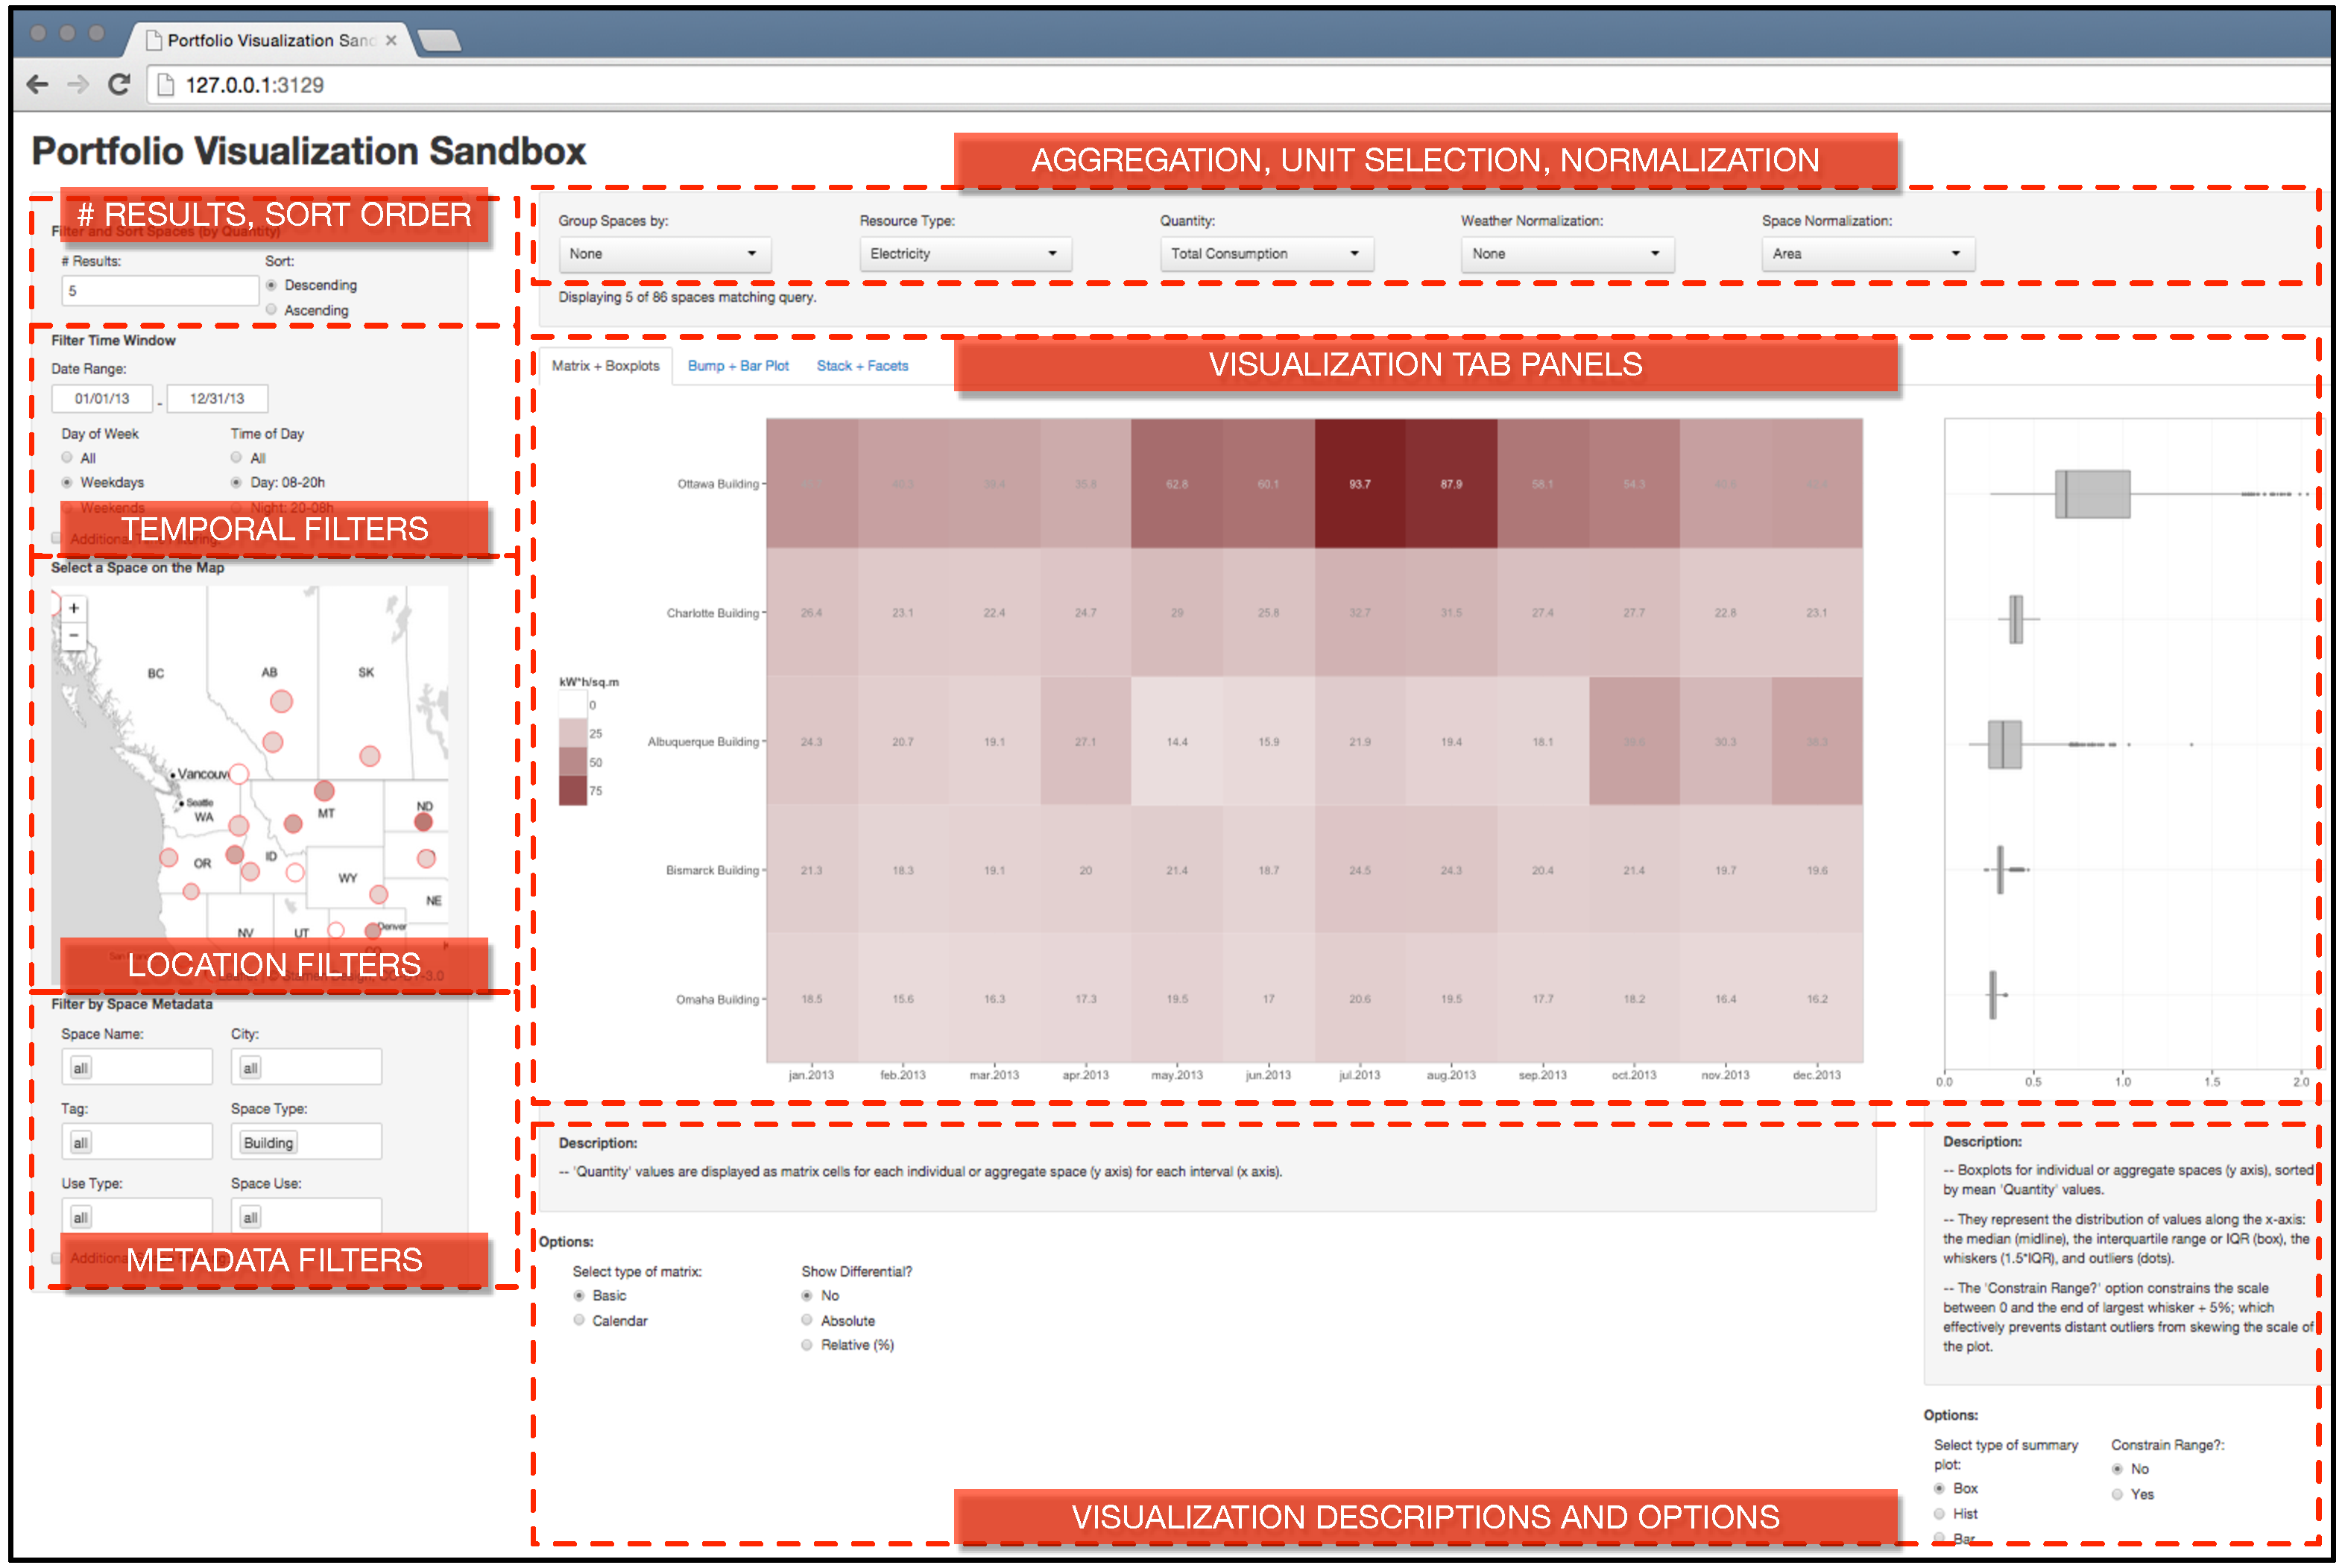
\includegraphics[width=\textwidth]{figures/sandbox.pdf}
	\vspace{-0.6cm}
	\caption{A browser-based design sandbox for visualizing energy data from a portfolio of buildings. Visualizations depicted in Figures~\ref{fig:sandbox-faceted-boxplot},~\ref{fig:sandbox-barbump},~\ref{fig:sandbox-calendar}, and~\ref{fig:sandbox-stacks} were also produced within this environment. Shown here is a matrix of aggregate \textsl{energy intensity} values with auxiliary boxplots.}
	\label{fig:sandbox}
% 	\vspace{-0.6cm}
\end{figure*} 

\bstart{Evaluating visualizations of time-oriented data} we also situate our work with regards to experimental studies~\cite{Albers2014,Fuchs2013,Javed2010} that have examined the viability of different visual encodings for abstract tasks similar to those that we characterized: identifying and comparing trends, extreme values, and outliers.
We too assessed the viability of different visual encodings, however our approach involves a qualitative evaluation with energy workers as opposed to a controlled experiment.

Albers~\etal~\cite{Albers2014} compared eight visual encodings of a single continuous time series for tasks in which the viewer is asked to identify one of seven aggregate values, such as the minima, maxima, average, or number of outliers. 
They do not examine the effectiveness of these encodings in faceted visualizations of multiple time series, which we address in the following section; specifically, we consider faceted line charts, boxplots, and colour stock charts.

As for multiple time series, Javed~\etal~\cite{Javed2010} compared the effectiveness of two superimposed encodings (a line chart and a braided graph) to two faceted encodings (small multiple line charts and horizon graphs) for data containing up to 16 concurrent time series.
Since our energy workers need to consider dozens to hundreds of concurrent time series, we are skeptical that their findings generalize to our situation, and we discuss alternative encodings in the following section. 
% Finally, Fuchs~\etal~\cite{Fuchs2013} evaluated four alternative faceted encodings for 48 concurrent time series.

These experiments~\cite{Albers2014,Fuchs2013,Javed2010} considered continuous time-series data, which is how we would characterize a building's raw {\it energy demand} or its {\it outdoor temperature}. 
As mentioned in Section~\ref{data-abstractions}, energy workers are accustomed to analyzing discrete derived and aggregated time series values corresponding to {\it energy consumption} or {\it intensity}.
A consequence of this domain convention is that any encoding that incorporates a line graph, including horizon charts~\cite{Heer2009}, are inappropriate and potentially misleading in our energy domain context.
Therefore, we need to consider scalable alternative encodings for time series of derived and aggregated values.

%-------------------------------------------------------------------------
%-------------------------------------------------------------------------

\section{Design and Evaluation}
\label{design}

%-------------------------------------------------------------------------
%-------------------------------------------------------------------------=

\bstart{Portfolio visualization sandbox} acknowledging the utility of interactive {\it data sketches} in visualization design~\cite{Lloyd2011}, we developed an interactive browser-based visualization design sandbox\footnote{\url{mattbrehmer.shinyapps.io/PortfolioSandbox}}, one where we could easily and rapidly prototype different visualization designs and demonstrate them to our collaborator and to external energy workers.
Most of the designs discussed in this section were produced within this environment (shown in Figure~\ref{fig:sandbox}), which was developed\footnote{\url{github.com/mattbrehmer/PortfolioSandbox}} using the Shiny web application framework\footnote{\url{shiny.rstudio.com}}.
Central to this sandbox environment are the interactive controls for filtering, aggregating, unit selection, and normalization; recall that there were no such controls in the {\it Energy Manager} interface.
% We deployed this visualization sandbox environment on our collaborator's local intranet. 
% It is also accessible publicly, though we had to use a small anonymized dataset for the latter due to client privacy concerns.

\bstart{Blocks and guidelines} we will analyze the visualizations that we considered with respect to the {\it Nested Blocks and Guidelines Model} by Meyer~\etal~\cite{Meyer2013}, which extends Munzner's {\it Nested Model}~\cite{Munzner2009,Munzner2014} and describes a need for guidelines that relate ``blocks'' at the domain, abstraction, idiom/technique, and algorithm levels.
Earlier in Section~\ref{abstractions}, we described the relationship between domain activity blocks and the data and task abstraction blocks.
In this section, we consider the space of techniques and present guidelines for matching idiom blocks to abstraction blocks. 
Since the space of possible visual encoding and interaction techniques is large~\cite{Aigner2011}, we undertook a typical design study approach~\cite{Sedlmair2012}: considering several techniques, implementing a subset of these, and ultimately selecting a few good matches based on an evaluation that coincided with our design process.

\bstart{Matches \& mismatches} we identified five matches between our abstract tasks ({\bf T1--T3}) and visualization idioms. 
We also identified four mismatches and one potential match. 
In the following subsections we describe our designs as well as why they constitute matches or mismatches; this is also summarized in Table~\ref{tab:matches-mismatches}.

Evidence for these matches and mismatches emanates from an evaluation that occurred alongside our design process, which involved both our collaborators and external energy workers.
% We defer a more detailed discussion of our methodological approach to this phase of the project until Section~\ref{discussion}.
Most of the design took place over the course of a four month period, and during this time we had weekly design feedback sessions with our collaborators.
We also conducted two 60--90 minute design feedback sessions with two external energy workers (4 individual sessions).
Both of these energy workers could be described as ``power users'' of {\it Energy Manager}, and we had previously spoken these individuals during the work domain analysis phase described in Section~\ref{domain}.
Finally, we conducted two additional feedback sessions with energy workers that we had not previously spoken to.
In each session, we asked energy workers about the perceived utility of our visualizations as well as how they might be used in the context of their energy analysis workflows.
We comment further on our methodological approach in this phase of the project in Section~\ref{discussion-methodology}. 
The following subsections reflect a subset of the findings from these sessions for each of the visualizations that we considered.

%-------------------------------------------------------------------------

\subsection{Faceted Visualizations for Overview and Detail Tasks}
\label{design-faceting}

%-------------------------------------------------------------------------'

%figure: faceting

We initially thought that faceted visualizations would be a good match for {\it both} the Overview ({\bf T1}) and Detail ({\bf T2}) tasks, and that faceting either by building or by temporal granularity provided a scalable alternative to grouped bar charts and superimposed line charts.

\bqstart{Faceted bar charts} were among the first designs to be considered, especially after one energy worker provided us with his own mockup of a faceted bar chart.
However, if an energy worker has dozens or hundreds of buildings in their portfolio, faceting is unlikely to scale~\cite{Javed2010}. 
We determined that it was a poor match for the Overview ({\bf T1}) task, though a potential match for the Detail ({\bf T2}) task, provided that the energy worker has already filtered down to a smaller group of buildings, such as filtering a university portfolio to show only the {\it ``classroom''} buildings.
In addition, one of the ``power user'' energy workers lamented that bars show only coarse aggregate values, typically an average or a sum, and as a result of this loss of detail, they do not show other aggregate values of interest, such as ranges or extreme values.

\begin{figure}[ht]
    % \vspace{-0.3cm}
	\centering
	\fbox{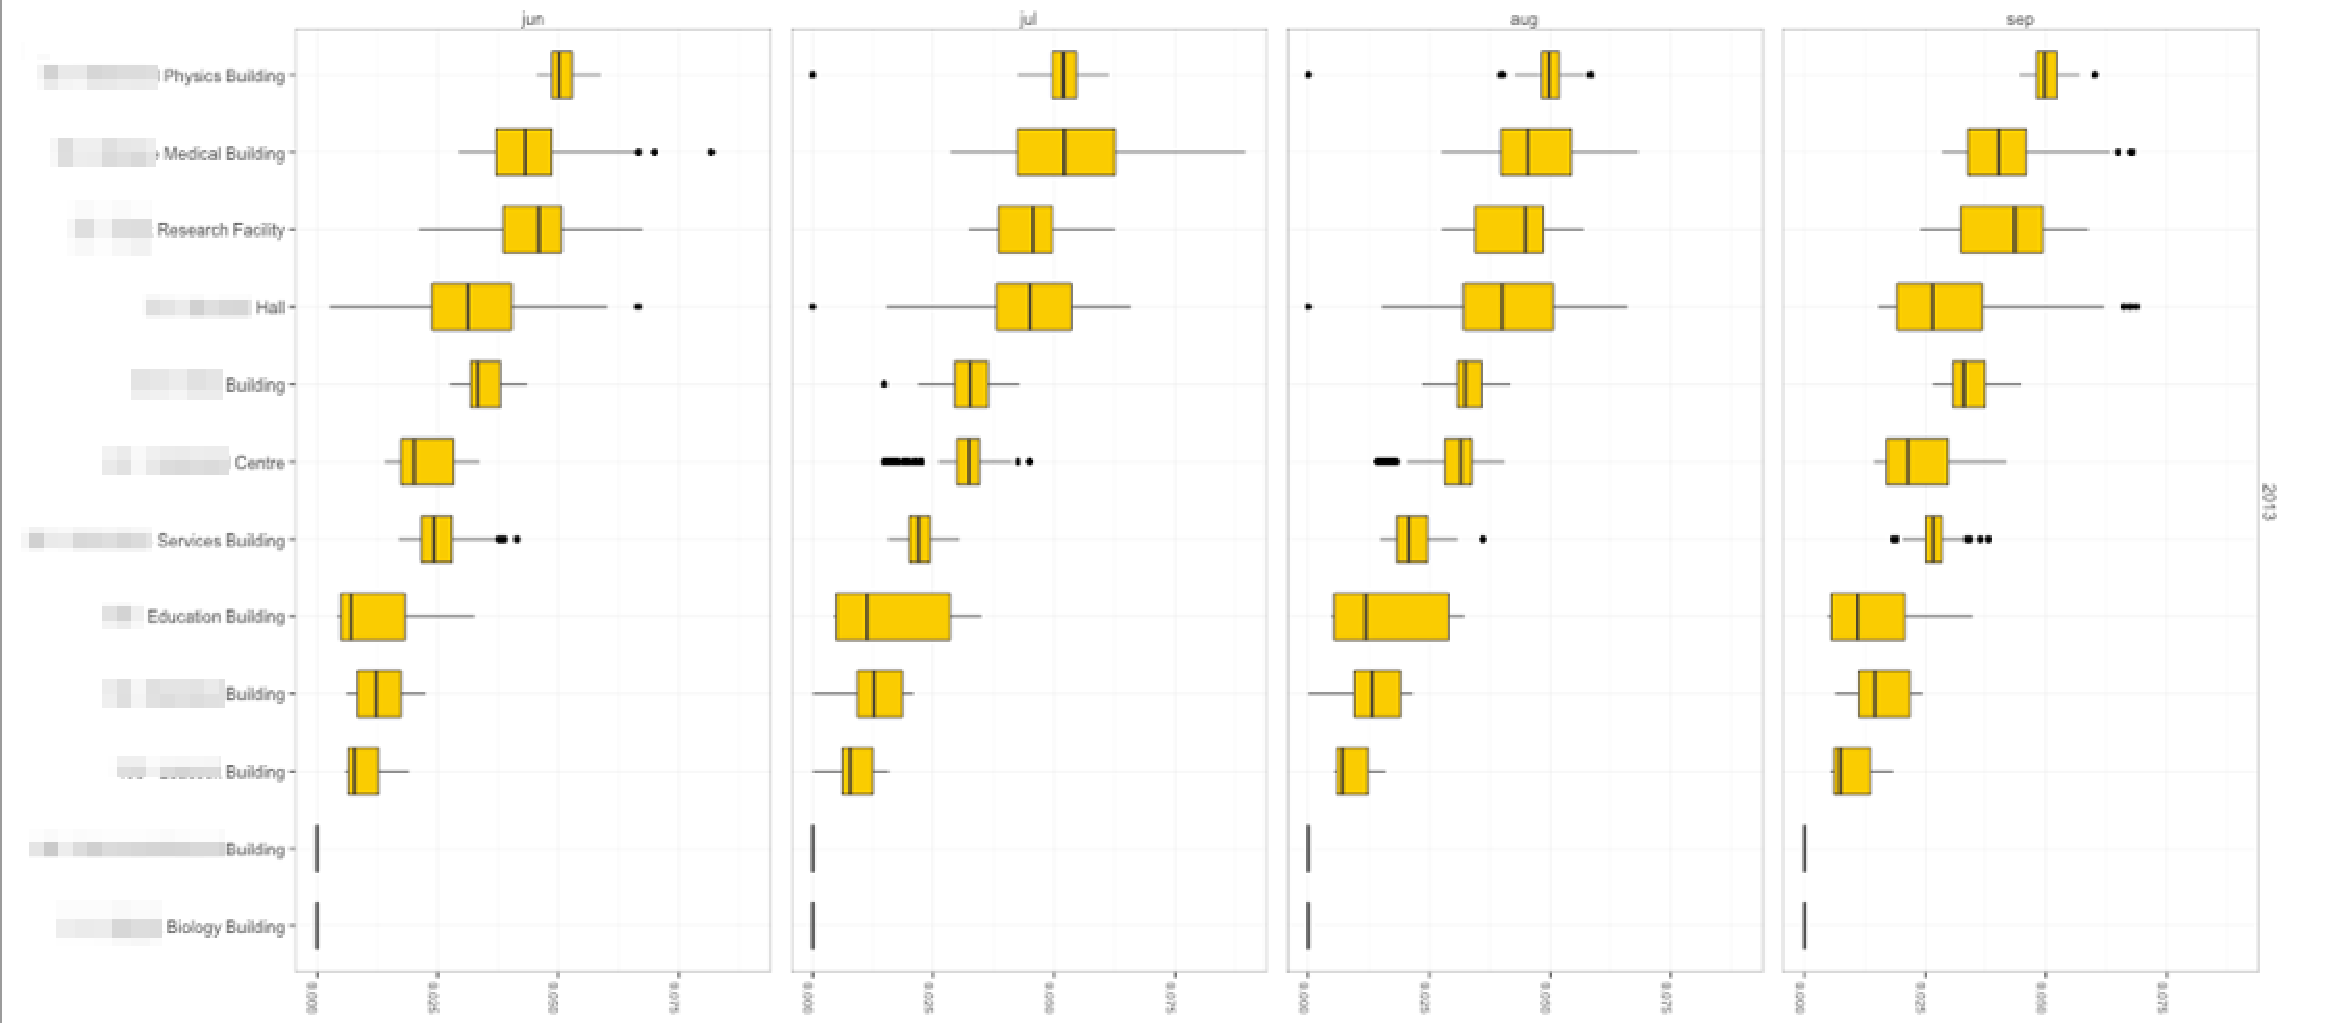
\includegraphics[width=0.95\columnwidth]{figures/sandbox-faceted-boxplot.pdf}}
	\vspace{-0.15cm}
	\caption{Faceted boxplots that encode aggregate energy performance values for 12 buildings across four months.}
	\label{fig:sandbox-faceted-boxplot}
	\vspace{-0.6cm}
\end{figure} 

\bqstart{Faceted boxplots} were the next design that we considered, as we expected that they would allow energy workers to compare ranges, distributions, and extreme values for multiple buildings at different points in time, such as in Figure~\ref{fig:sandbox-faceted-boxplot}.
However, despite their long history~\cite{Wickham2011} and support from influential visualization practitioners~\cite{Few2014}, we found that most energy workers are not familiar with boxplots, except for a minority who had taken a post-secondary statistics course.
Furthermore, unlike faceted bar charts where the observer must make comparisons of position aligned to a each facet's baseline: comparisons in faceted boxplots are more difficult because the observer are comparing multiple positions and widths across separate facets. 
Our design was therefore a daunting introduction to boxplots for those unfamiliar with them and a poor match for the Detail ({\bf T2}) task.

\bqstart{Faceted line charts}, however, are a good match for the Detail ({\bf T2}) task, especially when observing continuous quantitative time series values such as {\it energy demand} (as in Figure~\ref{fig:sandbox-stacks}), and they are a scalable alternative to superimposed line charts~\cite{Javed2010}. 
Furthermore, the line chart encoding is already very familiar to energy workers.

%-------------------------------------------------------------------------

\subsection{Overview Visualizations of Rank and Rank Change}
\label{design-ranking}

%-------------------------------------------------------------------------

As faceting seemed unlikely to be effective for the Overview ({\bf T1}) task, we considered non-faceted visualization of aggregate values.
Recall how the sortable table in {\it Energy Manager}'s portfolio dashboard (Figure~\ref{fig:energy-manager}-bottom left) was never used for the Overview ({\bf T1}) task; it contained only coarse aggregate values for each item, providing little detail about temporal variation.
We therefore experimented with encodings for displaying rank in addition to rank change over time.

\bqstart{Bump plots} are one such encoding; they incorporate a familiar line encoding across equally-spaced temporal intervals. 
However, as with superimposed line charts, it becomes difficult to distinguish individual items using colour.
One possible solution is to highlight items that vary in rank, rather than requiring the observer to locate these items.
Another problem is that bump plots only show relative rank and rank change, whereas the absolute values that produce these ranks are not shown. 
As a result this a loss of detail, the bump plot is also a poor match for the Overview ({\bf T1}) task.

\begin{figure}[ht]
    \vspace{-0.3cm}
	\centering
	\fbox{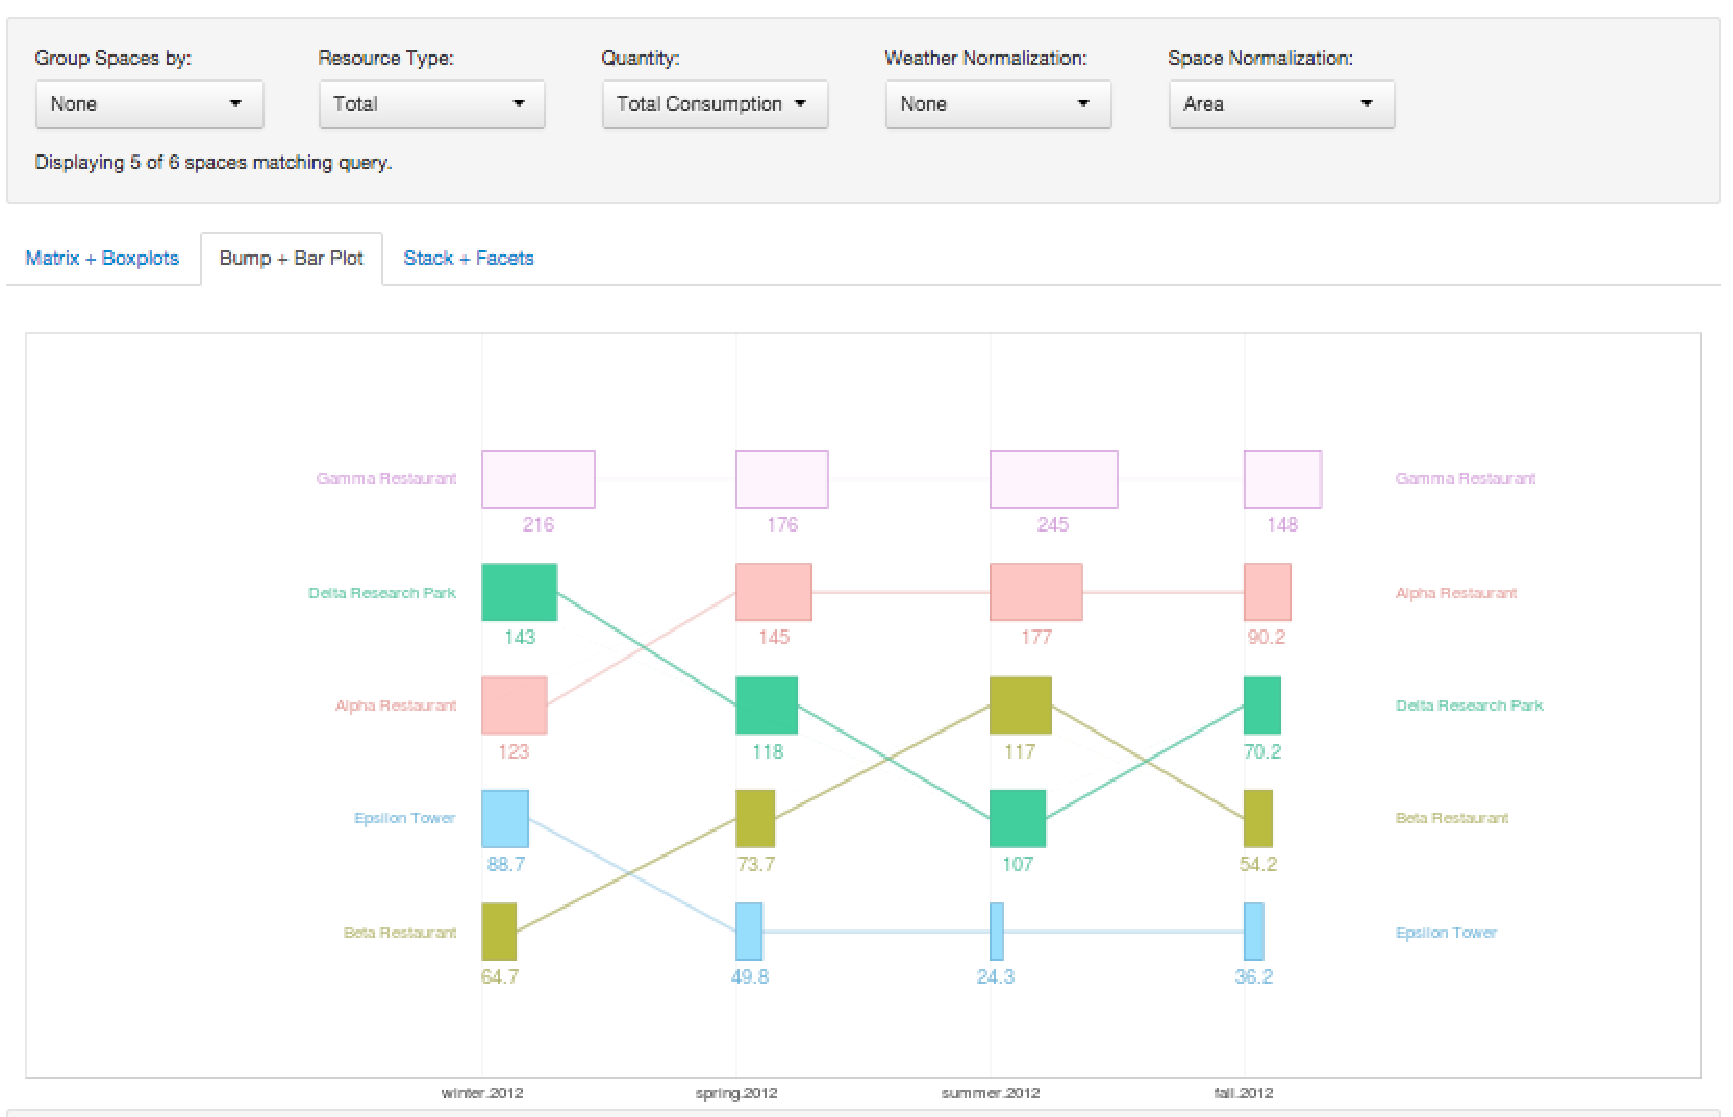
\includegraphics[width=0.95\columnwidth]{figures/sandbox-barbump.pdf}}
	\vspace{-0.15cm}
	\caption{A \textsl{bar + bump plot} of \textsl{energy intensity}, ranking five buildings across four seasons.}
	\label{fig:sandbox-barbump}
	\vspace{-0.3cm}
\end{figure}

\bstart{Bump + bar plots} we next considered an encoding that incorporates both relative rank, rank change, and absolute value, by adding familiar bars to each series in the bump plot, as shown in Figure~\ref{fig:sandbox-barbump}. 
This is similar to two recently proposed techniques that display both relative rank and absolute value~\cite{Gratzl2013,Hur2013}. 
With this design, we still face the scalability problem associated with colour discriminability.
A combination of interaction and highlighting by rank change or rank variation may facilitate this discriminability; in Figure~\ref{fig:sandbox-barbump}, rank variation is encoded using the alpha channel, so the green and gold series are most salient.
Energy workers responded positively to this visualization, as it is composed of familiar bar and line encodings. 
However despite this positive response, we discovered that {\it ranks} as derived values are actually infrequently considered during energy analysis, and that they tend to be more appropriate when energy workers {\it present} their findings to colleagues on a quarterly or annual basis.
Thus, the hunt for a match for the Overview ({\bf T1}) task continued.

%-------------------------------------------------------------------------

\subsection{Matrix-Based Overview Visualizations}
\label{design-matrix}

%-------------------------------------------------------------------------

%figure: matrix-based visualizations

% With faceting and rank-based designs proving ineffective, we next turned to a matrix-based encoding for the Overview ({\bf T1}) task.

\bqstart{Time series matrix} encodings such as in Figure~\ref{fig:sandbox} are scalable and space-efficient.
Matrix encodings allow us to display observed as well as differential values, allowing an energy worker to review {\it energy savings} relative to predicted or historical values; a matrix displaying differential energy data is shown in Figure~\ref{fig:sandbox-calendar}.
Most of the energy workers that we interviewed were unfamiliar with this form of encoding, except one who routinely made such visualizations in {\it Excel}. 
As a result, it took more effort to convince our collaborators of the value of these matrix-based encodings for the Overview ({\bf T1}) task.

We initially referred to these visual encodings as ``heat maps'', and this led to some confusion\footnote{This confusion is not unique to the energy domain~\cite{Field2015,Wilkinson2009}.}, as {\it heat} is already an energy-related word and buildings have a location, though this encoding does not take spatial location into account.
We also discovered that while red is fine for use in diverging colour scales, as it has a negative connotation, and is therefore inappropriate for unidirectional colour scales. 
Finally, we learned that energy workers found matrices with diverging colour scales easier to interpret than than those with unidirectional colour scales.
As a result of this mixed response to matrix-based encodings, we realized that more work needed to be done.

\begin{figure}[ht]
    \vspace{-0.15cm}
	\centering
	\fbox{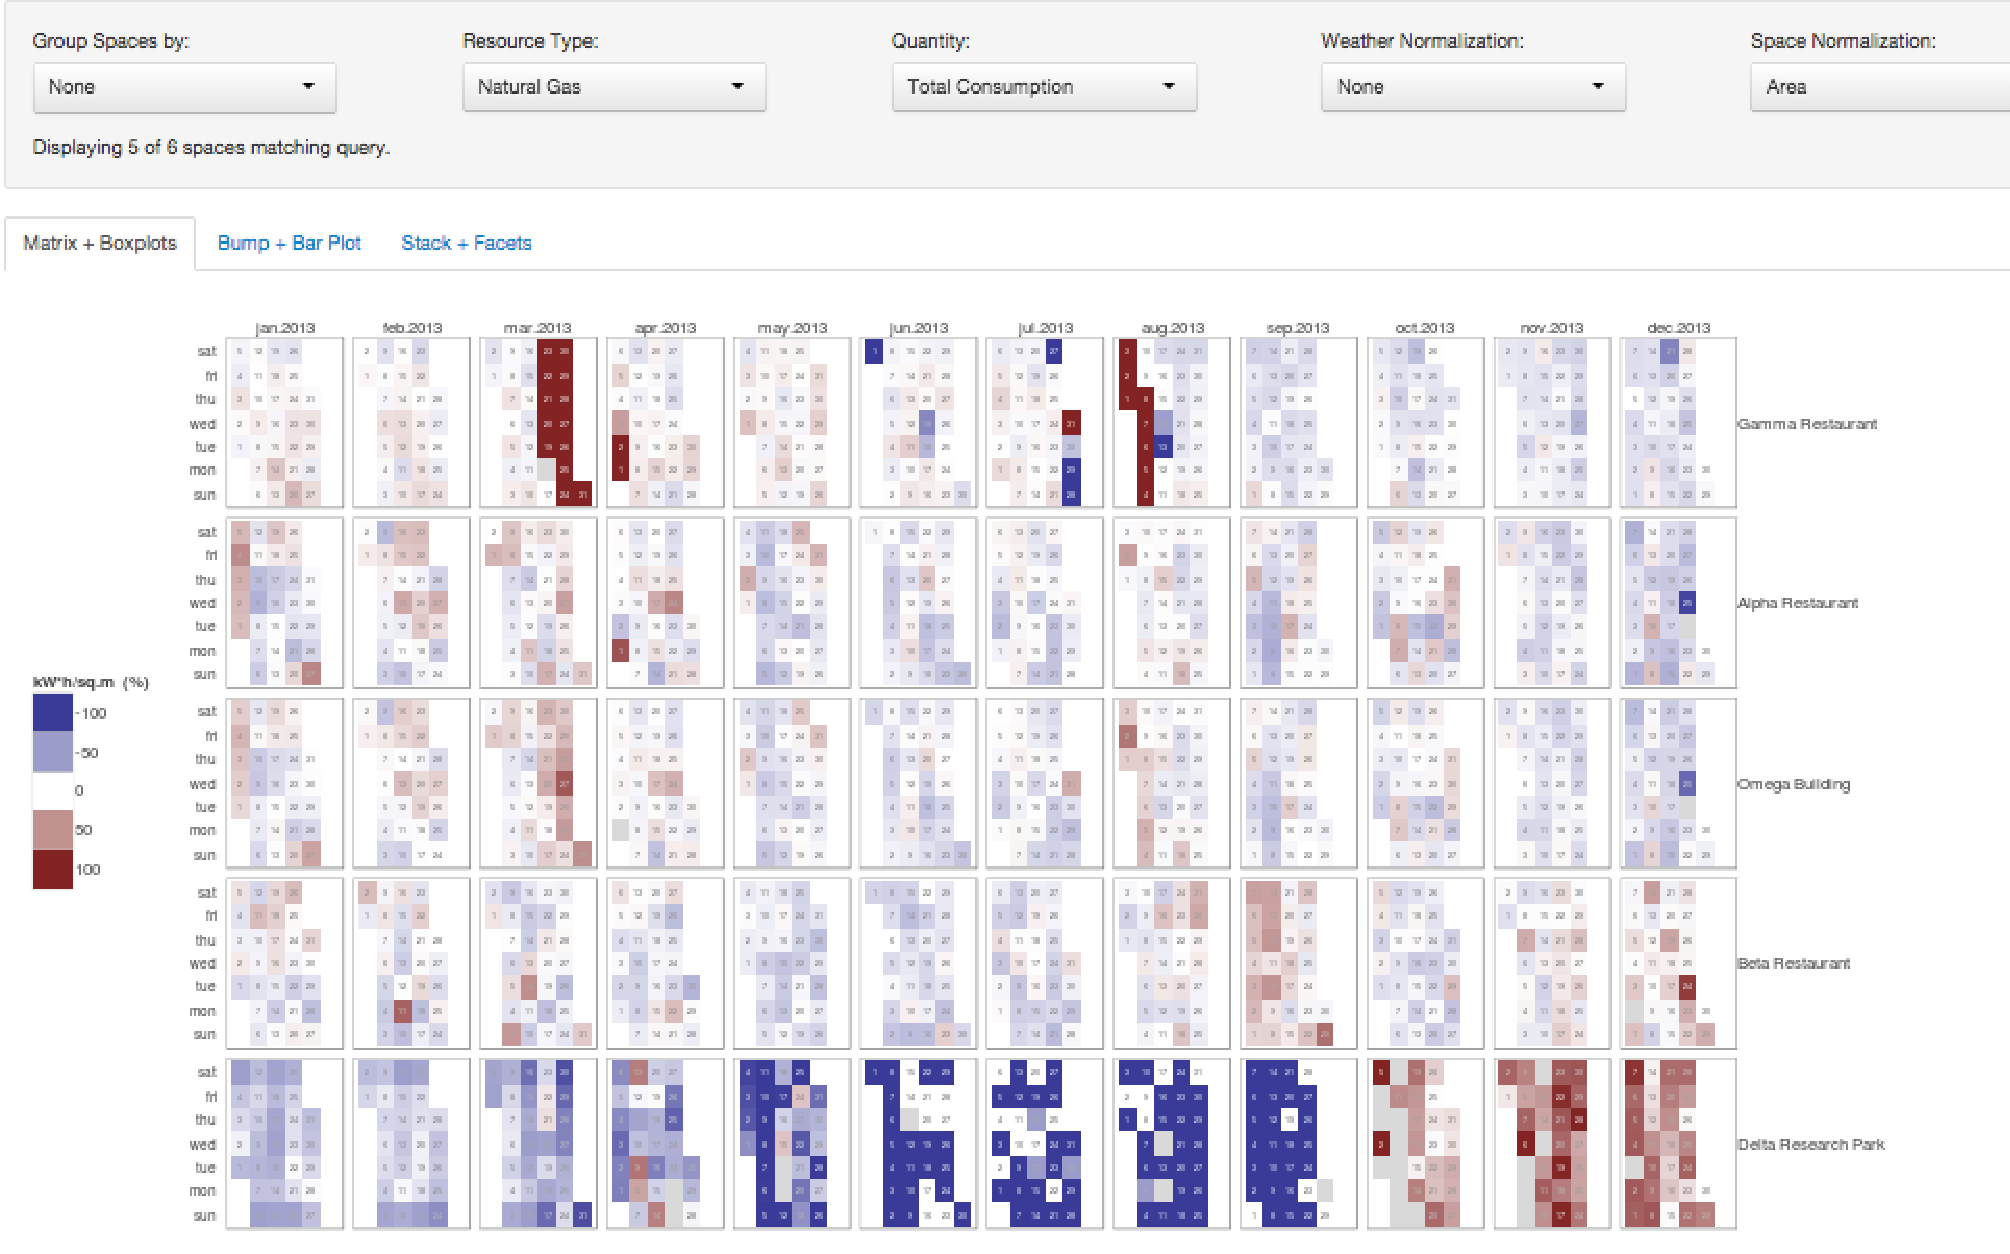
\includegraphics[width=0.95\columnwidth]{figures/sandbox-calendar.pdf}}
	\vspace{-0.15cm}
	\caption{A time-series calendar matrix of \textsl{energy intensity savings} for five buildings, relative to historical values (blue = \textsl{savings}).}
	\label{fig:sandbox-calendar}
	\vspace{-0.3cm}
\end{figure}

\bstart{Calendar matrix} we altered our matrix encoding by partitioning the cells corresponding to months into calendars (Figure~\ref{fig:sandbox-calendar}), a design decision inspired by previous work~\cite{vanWijk1999}. 
Energy workers responded positively to this encoding, indicating this helped to resolve the unfamiliarity of the matrix encoding.

\bstart{Matrix with auxiliary boxplots} a problem with the matrix encodings is that they display coarse aggregate values only: averages or sums for each matrix cell. 
Calendar partitioning is one way to show a finer resolution in the same amount of space. 
In addition, we can complement the aggregate values in the matrix by juxtaposing boxplots that encode ranges and distributions for each time series, as shown in Figure~\ref{fig:sandbox}.
Though boxplots remain unfamiliar, these auxiliary boxplots are easier to interpret than faceted boxplots (such as in Figure~\ref{fig:sandbox-faceted-boxplot}), and they are reinforced by the aggregate values shown the adjacent matrix. 
As a result, we decided that a matrix with juxtaposed auxiliary boxplots is a match for the Overview ({\bf T1}) task.

%-------------------------------------------------------------------------

\subsection{Proportion Visualizations}
\label{design-proportion}

%-------------------------------------------------------------------------

%figure: proportion visualizations

\bstart{Stacked area \& bar charts} With the Overview ({\bf T1}) and Detail ({\bf T2}) tasks addressed, the Proportion ({\bf T3}) task remains. 
The visualization for this task tended to be more obvious, with stacked area and stacked bar charts appearing to be likely matches.
However, recall that the Detail ({\bf T2}) and Proportion ({\bf T3}) tasks are often performed in alternation, so we were concerned about the loss of context when switching between stacked bar or area charts and faceted bar or line charts.

\begin{figure}[ht]
    \vspace{-0.15cm}
	\centering
	\fbox{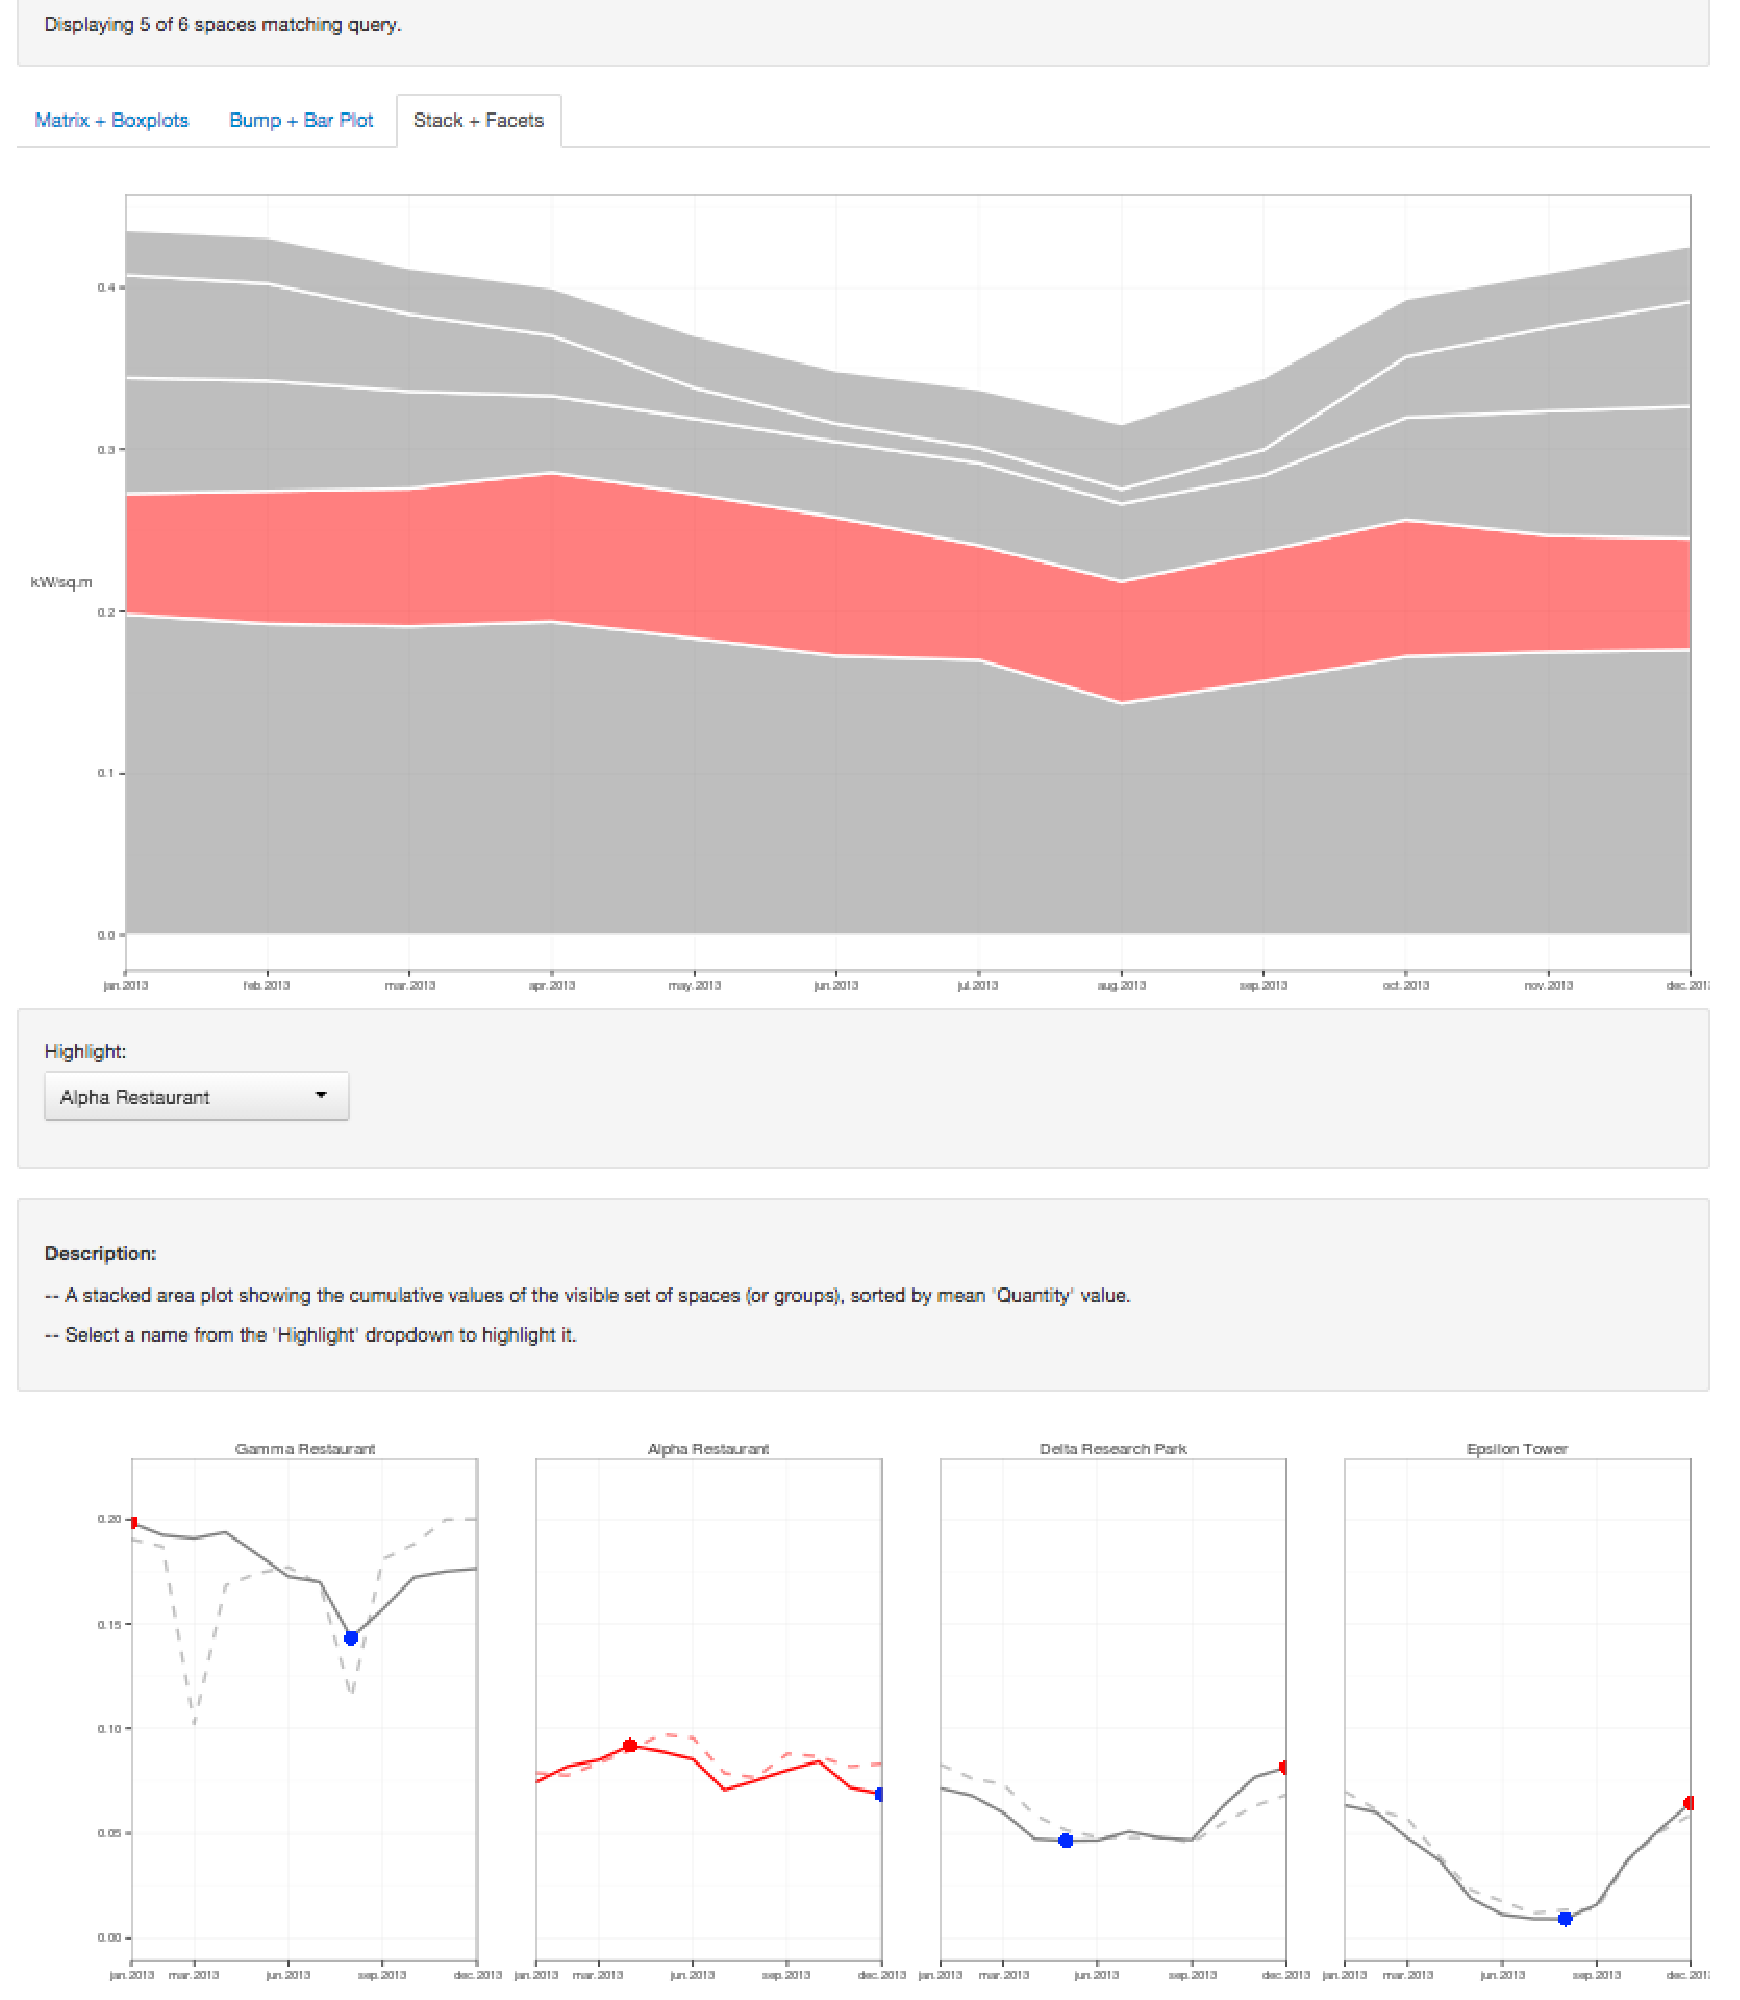
\includegraphics[width=0.95\columnwidth]{figures/sandbox-stacks.pdf}}
	\vspace{-0.15cm}
	\caption{A stacked area chart of \textsl{energy demand} data for five buildings, juxtaposed alongside faceted line charts of the same data. The dashed line in each facet encodes historical values for the previous year. The ``Alpha restaurant'' building is highlighted in both encodings.}
	\label{fig:sandbox-stacks}
	\vspace{-0.45cm}
\end{figure}

\bstart{Juxtaposed stacked and faceted visualizations} to prevent a loss of context when alternating between the Detail ({\bf T2}) and Proportion ({\bf T3}) tasks, we juxtaposed the stacked chart with the faceted charts, and provide linked highlighting between elements in the stack and those in the facets, such as in Figure~\ref{fig:sandbox-stacks}. 
As a result of this juxtaposition and linked highlighting, both the Detail ({\bf T2}) and Proportion ({\bf T3}) tasks are supported in a single display.

%-------------------------------------------------------------------------

\subsection{Summary of Matches and Mismatches} 
\label{design-summary}

%-------------------------------------------------------------------------

We identified five matches between abstract tasks ({\bf T1--T3}) and visualization idioms. 
We also identified four mismatches and one potential match: that of a {\it bump + bar plot} for showing rank change over time; our hesitation to call this a match stems not from a problem with the visualization itself, but from energy workers' low priority on ranks as derived data of interest.
These matches and mismtaches are summarized in Table~\ref{tab:matches-mismatches}.

\begin{table}[ht]\renewcommand{\arraystretch}{1.2}\addtolength{\tabcolsep}{-1pt}
    % \vspace{-.15cm}
    \begin{center}
    \scriptsize
    \begin{tabular}{l|l|c}

        \rowcolor{gray!15}
    
        {\bf Task} & {\bf Visualization Idiom} & {\bf Match?}
        
        \\
        
        %task
        \cellcolor{nmYellow} {\bf T1}: Overview 
        
        %idiom
        & \cellcolor{nmGreen} Faceted bar chart 
        
        %match?
        & \mismatch
        
        \\
        
        %task
        \cellcolor{nmYellow} %{\bf T1}: Overview 
        
        %idiom
        & \cellcolor{nmGreen} Bump plot 
        
        %match?
        & \mismatch
        
        \\
        
        %task
        \cellcolor{nmYellow} %{\bf T1}: Overview 
        
        %idiom
        & \cellcolor{nmGreen} Bar + bump plot 
        
        %match?
        & \posmatch
        
        \\
        
        %task
        \cellcolor{nmYellow} %{\bf T1}: Overview 
        
        %idiom
        & \cellcolor{nmGreen} Map 
        
        %match?
        & \mismatch
        
        \\
        
        %task
        \cellcolor{nmYellow} %{\bf T1}: Overview 
        
        %idiom
        & \cellcolor{nmGreen} (Calendar) matrix 
        
        %match?
        & \posmatch
        
        \\
        
        %task
        \cellcolor{nmYellow} %{\bf T1}: Overview 
        
        %idiom
        & \cellcolor{nmGreen} Matrix + auxiliary boxplots 
        
        %match?
        & \match
        
        \\
        
        \hline
        
        %task
        \cellcolor{nmYellow} {\bf T2}: Detail 
        
        %idiom
        & \cellcolor{nmGreen} Faceted bar chart 
        
        %match?
        & \match
        
        \\
        
        %task
        \cellcolor{nmYellow} %{\bf T2}: Detail 
        
        %idiom
        & \cellcolor{nmGreen} Faceted boxplot 
        
        %match?
        & \mismatch
        
        \\
        
        %task
        \cellcolor{nmYellow} %{\bf T2}: Detail 
        
        %idiom
        & \cellcolor{nmGreen} Faceted line graph 
        
        %match?
        & \match
        
        \\
        
        \hline
        
        %task
        \cellcolor{nmYellow} {\bf T3}: Proportion 
        
        %idiom
        & \cellcolor{nmGreen} Stacked area graph 
        
        %match?
        & \match
        
        \\
        
        %task
        \cellcolor{nmYellow} %{\bf T3}: Proportion 
        
        %idiom
        & \cellcolor{nmGreen} Stacked bar chart 
        
        %match?
        & \match
        
        \\
        
        \hline  
        
    \end{tabular}
    \vspace{-0.3cm}
    \caption{A summary of the \textsl{matches} and \textsl{mismatches} between abstract tasks and visualization idioms.}
    \label{tab:matches-mismatches}
    \end{center}
    \vspace{-0.6cm}
\end{table}

Considering how we abstracted these energy analysis tasks and discussed their similarity to tasks addressed in previous work~\cite{Albers2014,Javed2010}, these five matches between visualization idioms and abstract tasks serve as generalizable guidelines that are transferable beyond the energy domain.
Furthermore, these guidelines fill a gap with regards to identifying visualization idioms for multiple time series in which the values are not continuous, but derived and aggregated values that {\it should not} be represented using (faceted) line or horizon charts~\cite{Heer2009}.

%-------------------------------------------------------------------------

\subsection{Interaction Design Considerations}
\label{design-interaction}

%-------------------------------------------------------------------------

The design discussion up until this point has been largely about visual encoding choices. 
We also want to stress the importance of interaction idioms in support of the abstract tasks characterized above.
The visualization sandbox environment allowed us to easily explore the design space of visual encodings, as well as interactions involving filtering, aggregation, and deriving normalized values.
However, our implementation did not allow us to investigate interactions involving coordinated selection, linking, and brushing across for juxtaposed visualizations, nor did it allows us to easily prototype interactive drill-down behaviour from Overview ({\bf T1}) to Detail ({\bf T2}) and Proportion ({\bf T3}) visualizations.

\begin{figure}[ht]
    \vspace{-0.3cm}
	\centering
	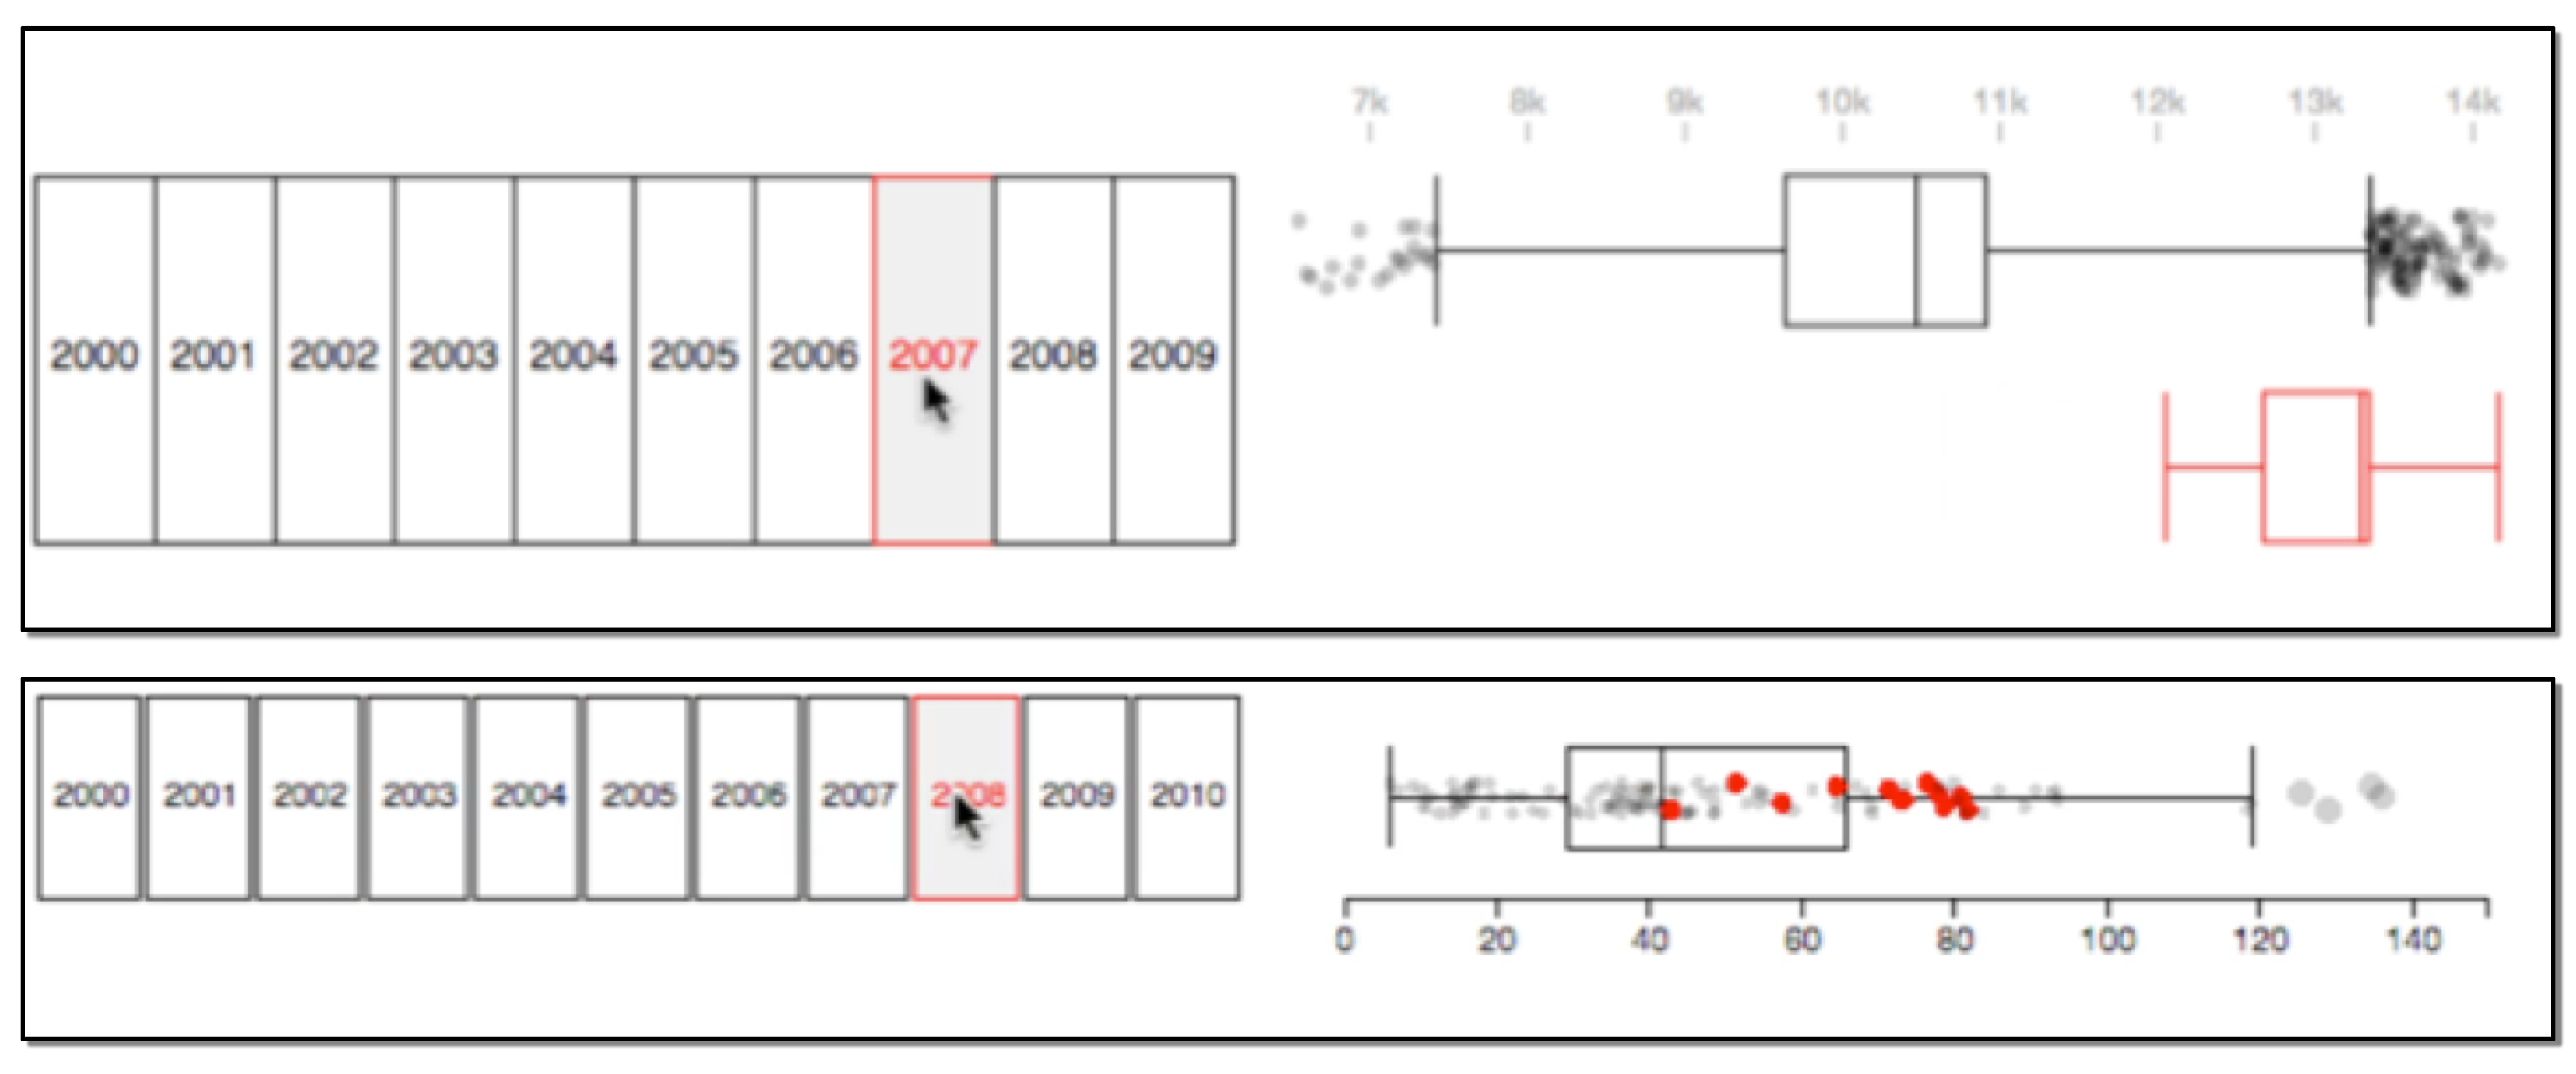
\includegraphics[width=\columnwidth]{figures/d3-boxplots.pdf}
	\vspace{-0.6cm}
	\caption{Two interactive auxiliary boxplot alternatives. Top: values corresponding to the brushed time period are superimposed as jittered points on the boxplot. Bottom: boxplots corresponding to the brushed time period are shown alongside the boxplot for the entire time series.}
	\label{fig:interactive-boxplots}
	\vspace{-0.3cm}
\end{figure}

\begin{figure*}[ht!]
    % \vspace{-0.6cm}
	\centering
	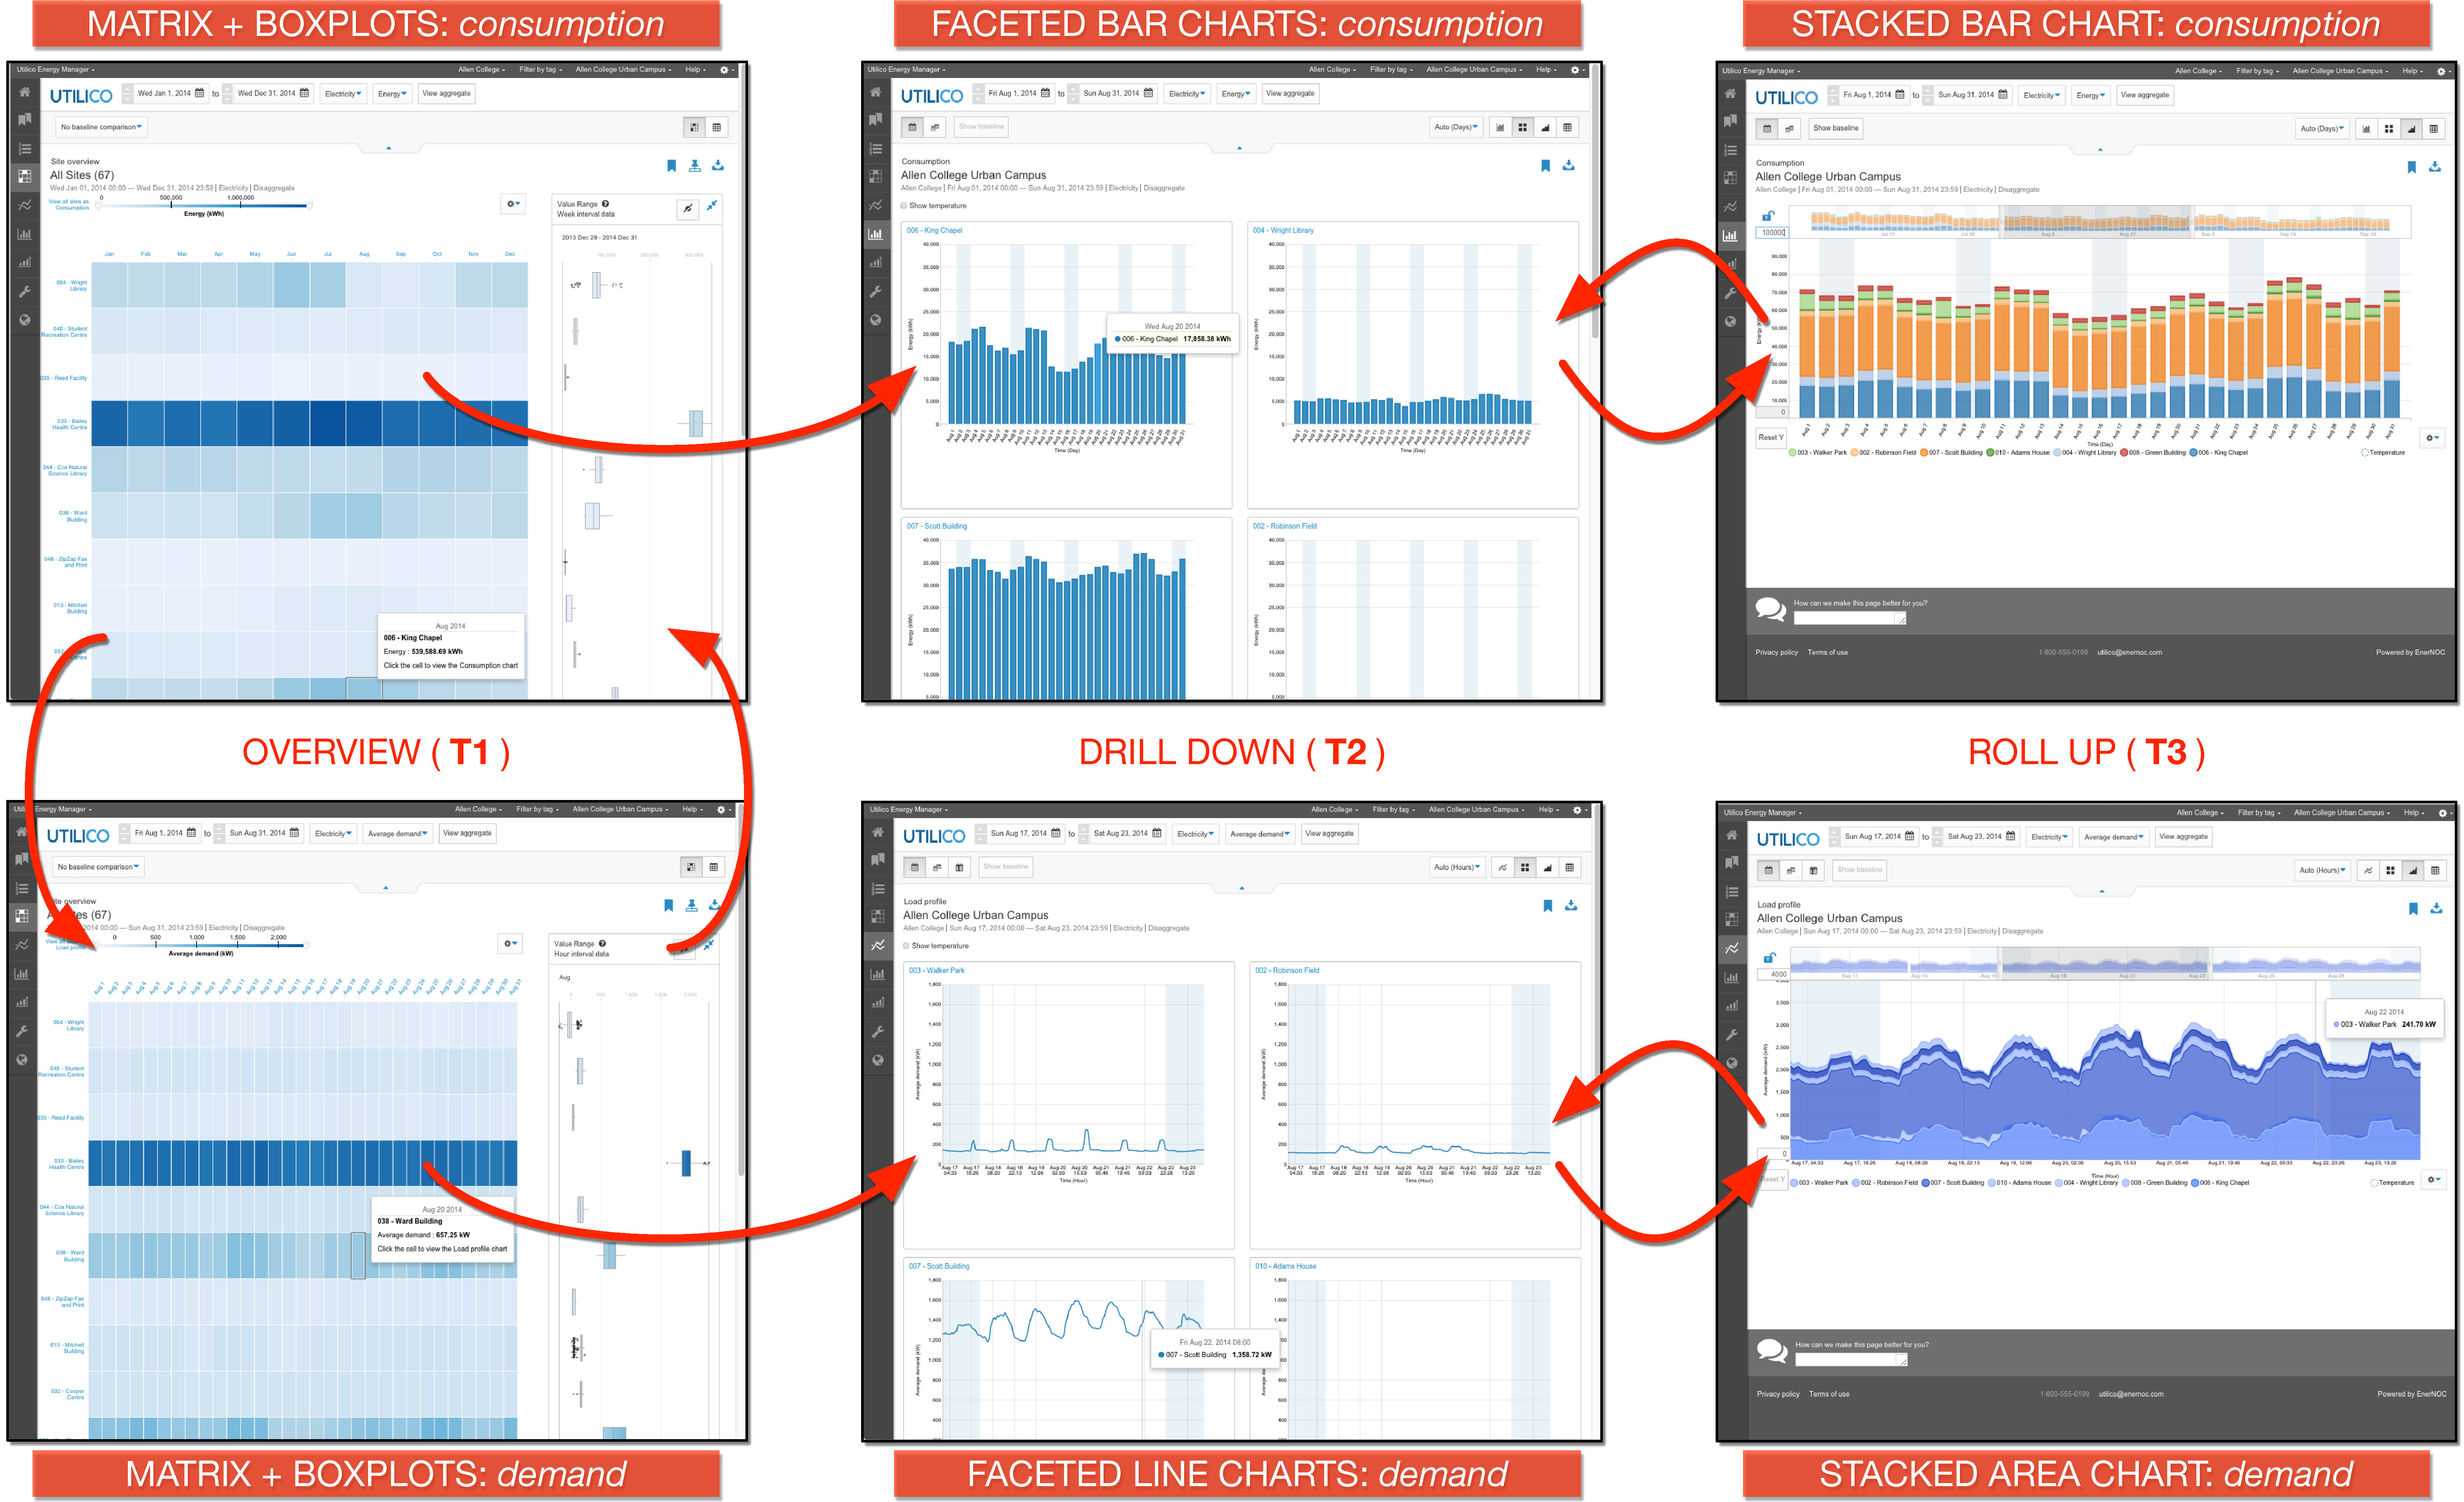
\includegraphics[width=\textwidth]{figures/emu.pdf}
	\vspace{-0.6cm}
	\caption{A redesigned \textsl{Energy Manager} which incorporates many aspects of our prototype designs. On the left, the \textsl{Site Overview} (a time series matrix) is juxtaposed with coordinated \textsl{Value Range} (boxplot) visualizations. An energy worker can easily switch between units such as \textsl{energy consumption} or \textsl{energy demand} and filter the set of buildings to those that share a common categorical tag; she can then drill-down to faceted or stacked visualizations of \textsl{ consumption} (top right) or \textsl{ demand} (bottom right) by selecting a column of the matrix.}
	\label{fig:emu}
	\vspace{-0.6cm}
\end{figure*} 

\bstart{Interactive auxiliary boxplots} we sought a better way to coordinate the time series matrix and its juxtaposed auxiliary boxplots.
Two interactive prototypes\footnote{\url{bl.ocks.org/mattbrehmer/8be29724bdd7a63ff41d}}$^,$\footnote{\url{bl.ocks.org/mattbrehmer/287e44c9a12151967874}}, shown in Figure~\ref{fig:interactive-boxplots}, were developed using D3.js~\cite{Bostock2011}.
The interactive linked highlighting in these prototypes served both to promote engagement with the visualizations and to facilitate the learning of these visual encodings, which were previously unfamiliar to energy workers. 
These prototypes further convinced our collaborators that a time series matrix with juxtaposed auxiliary boxplots was a good match for the Overview ({\bf T1}) task.

\bstart{Interactive drill-down} drawing upon visualizations created using our sandbox environment, mockups, and feedback from energy workers, we produced storyboards to describe how an energy worker would proceed from the Overview ({\bf T1}) task, being performed with the matrix and auxiliary boxplots, to the Detail ({\bf T2}) and Proportion ({\bf T3}) tasks, being performed with the faceted and stacked bar and line charts.
These storyboards, along with our consolidated findings from the feedback sessions with energy workers, were presented to our collaborators to help them decide whether they should incorporate our designs into production development, and in which priority.

%-------------------------------------------------------------------------
%-------------------------------------------------------------------------

\section{Results: Production}
\label{production}

%-------------------------------------------------------------------------
%-------------------------------------------------------------------------

We are pleased to report that our collaborators adopted a number of our visualization designs into a new version of {\it Energy Manager}, shown in Figure~\ref{fig:emu}, which will soon be deployed to its large user base.
The user base is also expected to grow dramatically as a result of their recent partnership with a large utility company: many thousands of energy workers will now be able to analyze the energy performance of their building portfolios with the redesigned {\it Energy Manager}.

As in our sandbox environment, options filtering and aggregating buildings according to shared categorical tags are now prominently in the top menu bar of the interface. 
They also provided the ability for energy workers to select units of interest and compare observed energy values against trusted historical values, as an alternative to comparing observed values to less trusted predicted values generated by a statistical model, which was a limitation of the original {\it Energy Manager}.

\bqstart{Coordinated matrix and boxplots} have been incorporated into the redesign {\it Energy Manager}; the matrix is labeled as a ``site overview'', which avoids the ``heat map'' misnomer, and corresponds well with our characterization of the ``Overview'' ({\bf T1}) task. 
% Our collaborators also added the ability to interactively adjust the colour scale bounds of the matrix.
Our collaborators did consider the alternative calendar-based encoding, however because they also intend for the redesigned {\it Energy Manager} to be accessible on a tablet (a requirement which arose later in the design process), partitioning the matrix cells into calendars may result in calendar dates too small to be selectable without form of zooming, which may incur a high implementation cost.
Meanwhile, the boxplots, now referred to as ``Value range'' visualizations, update when the energy worker brushes a cell in the corresponding matrix row, similar to the behaviour of the prototypes we described in Section~\ref{design-interaction}. 

\bstart{Interactive drill-down realized} another critical improvement over the original {\it Energy Manager} is the ability for an energy worker to drill down from a row, column, or cell of the matrix to stacked, faceted, superimposed, or individual line and bar charts, thereby accelerating the sequence from the Overview ({\bf T1}) task to the Detail ({\bf T2}) and Proportion ({\bf T3}) tasks.
Stacked views and faceted views are currently shown separately; are collaborators are considering juxtaposing stacked and faceted visualizations, such as in the design described in Section~\ref{design-proportion}, which would allow for uninterrupted alternation between the Detail ({\bf T2}) and Proportion ({\bf T3}) tasks.

%-------------------------------------------------------------------------
%-------------------------------------------------------------------------

\section{Discussion}
\label{discussion}

%-------------------------------------------------------------------------
%-------------------------------------------------------------------------

We now step back from specific aspects of visualization design to discuss higher-level guidelines and our methodology.

%-------------------------------------------------------------------------

\subsection{Guidelines}
\label{discussion-guidelines}

%-------------------------------------------------------------------------

In addition to the specific guidelines regarding matches and mismatches between idioms and abstractions described in Section~\ref{design}, we also propose more general and succinct guidelines relating to the themes of {\it familiarity} and {\it trust}.

\bstart{Familiarity}.
As with professionals in many other domains, energy workers are accustomed to working predominantly with familiar visual encodings, namely bars and lines.
When we introduced them to unfamiliar visualization designs, we learned several things:

{\it Complexity can reduce unfamiliarity}: paradoxically, we learned that adding complexity increased interpretability; the juxtaposition of a matrix and a boxplot, two unfamiliar encodings, together with coordinated interaction and highlighting, received more positive feedback than either of these encodings in isolation.
Similarly, energy workers indicated that the more complex diverging colour scales for derived {\it savings} values were easier to interpret than the simpler unidirectional colour scales for observed {\it energy consumption} values. %, or how providing the ability to adjust the colour scale bounds improved matrix interpretation.

{\it Familiarity is additive}: familiar encodings, such as bars and lines, can be combined in unfamiliar ways, such as in the {\it bump + bar plot}, and that these novel combinations are easily interpreted.

{\it Take care with names}: names for unfamiliar visual idioms can be misleading: ``heat map'' ~\cite{Field2015,Wilkinson2009} and ``boxplot''~\cite{Wickham2011} were particular sources of confusion that we encountered.
In introducing these unfamiliar visualizations, we primed the energy workers to think in a certain way, prompting expectations about the values being encoded. 
In hindsight, we could have explicitly solicited energy workers for visualization names based on their own descriptions~\cite{Metoyer2012}.

\bqstart{Trust} in a visualization is central part of the hypothesis generation and verification process. 
Previous work has investigated the trustworthiness of visualizations for text-based data~\cite{Chuang2012}, and we now discuss the topic of trust as it relates to visualizations of multiple time series:

{\it Auxiliary boxplots to combat loss of information}: when the number of concurrent time series grows large, it is difficult and overwhelming to visualize individual values from each time series; instead, a common approach is to visualize derived aggregate values~\cite{McLachlan2008}.
This loss of detail is apparent in the original {\it Energy Manager}'s portfolio dashboard (Figure~\ref{fig:energy-manager}) as well as in the cells of our time series matrix (Figure~\ref{fig:sandbox}).
Whenever there is a loss of detail, there is a loss of trust: one of the ``power user'' energy workers remarked that these derived aggregate values hide information such as extreme values.
In juxtaposing the time series matrix with auxiliary boxplots that update whenever a matrix cell containing an aggregate value is brushed,  we are not only restoring lost information: we are also restoring trust.

{\it Promote agency over derived values}: in our sandbox environment and in the redesigned {\it Energy Manager}, we provided explicit and obvious interactive controls for filtering, aggregation, normalization, and unit selection, controls that were missing in the original {\it Energy Manager}.
With these controls, we provide energy workers agency over the creation of derived values, these values become more trusted.
Similarly, the redesigned {\it Energy Manager} includes the option to compare observed energy performance to selected historical values, as an alternative to comparing against predicted values generated by a statistical model; until there is some visual indication as to how model values were generated, there will be little trust, and it is therefore preferable to allow the observer to select trusted historical values.

%-------------------------------------------------------------------------

\subsection{Methodological Considerations}
\label{discussion-methodology}

%-------------------------------------------------------------------------

This project involved several phases, with different methods employed and multiple research artefacts generated at each phase, which we summarize in Table~\ref{tab:methodology}.
Though our overall approach is similar to many other visualization design studies~\cite{McKenna2014,Sedlmair2012}, there are some specific aspects of our methodology that are unique to projects executed in company settings~\cite{Sedlmair2011}, and those involving remote prospective visualization users~\cite{Brehmer2014a}.

\begin{table}[ht]\renewcommand{\arraystretch}{1.2}\addtolength{\tabcolsep}{-1pt}
    \vspace{-.3cm}
    \begin{center}
    \scriptsize
    \begin{tabular}{l|*{4}l}
    
        \rowcolor{gray!15}
    
        & \multicolumn{4}{c}{\bf Artefacts}
        
        \\

        \rowcolor{gray!15}
    
        {\bf Phase} & \rot{slides, demos} & \rot{interviews} & \rot{annotations} & \rot{summary}
        
        \\
        
        \hline  
        
        (i) Work domain analysis & & \OK & & \OK
        
        \\
        
        (ii) Define and verify abstractions & \OK & \OK & \OK & \OK
        
        \\
        
        (iii) Develop visualization sandbox & \OK & & & \OK
        
        \\
        
        (iv) Evaluate visualizations, consider workflows & \OK & \OK & \OK & \OK
        
        \\
        
        (v) Prototyping specific interactions & \OK & & & 
        
        \\
        
        (vi) Production coding by collaborator & \OK & \OK & \OK &
        
        \\
        
    \end{tabular}
    % \vspace{-0.3cm}
    \caption{Phases of our methodology and associated research artefacts.}
    \label{tab:methodology}
    \end{center}
    \vspace{-0.6cm}
\end{table}

\bstart{Work domain analysis} conducting a rigorous and systematic work domain analysis can be time consuming and logistically challenging.
However, it is helpful to realize that authorities on work domain analysis~\cite{Vicente1999} established their methodologies in the design of high-risk, high-cost systems, such as nuclear power plant control rooms.
Work domain analysis and requirements analysis methodologies for many visualization design projects can be more flexible and creative~\cite{Goodwin2013,McNamara2014}.

\bqstart{Slide decks as research artefacts} following the work domain analysis phase, we consolidated our notes and screenshots in an annotated slide deck, which we made available to our collaborator.
Once we had characterized our data and task abstractions, we validated these abstractions with two ``power user'' energy workers. 
To do so, we again used slide decks to present and define the abstractions along with examples, screenshots, and mockups incorporating data from their own portfolio. 
We later annotated these slide decks with their feedback.
Similarly, feedback from collaborators and energy workers during the design phase was consolidated in a master slide deck and presented to our collaborator as evidence-based design recommendations.
Slide decks are an inherently effective way to explain visual encodings, as well as potential interactions using animations and slide transitions; they are also easy to share, especially with remote stakeholders.

\bqstart{Remote stakeholders} contributed to the logistical complexity of each phase of our project. 
Since many of the energy workers we consulted with are located in other cities or countries, many methods for requirements analysis and participatory design~\cite{Goodwin2013,McKenna2014} that depend on the researchers and stakeholders being co-located cannot be implemented~\cite{Brehmer2014a}.
As a result, we relied heavily on videoconferencing, screen sharing, and screen capture software.
For each feedback session with energy workers during the project's design and evaluation phase, we created a personalized slide deck which included screenshots from our sandbox environment along with explanations; these slides were sent to energy workers in advance.
During these sessions, we shared our screen to demonstrate designs from our visualization sandbox.
Recognizing the importance of showing project stakeholders their own data~\cite{Lloyd2011}, both the slide decks and the demonstrations would feature data from the energy worker's own portfolio of buildings.
Feedback from these sessions were recorded as annotations on the same slide decks.

\bstart{Corporate stakeholders} Sedlmair~\etal~\cite{Sedlmair2011} discussed methodological considerations for visualization design and evaluation in corporate settings, and we certainly faced many of the challenges that they identified. 
Many visualization design collaborations between academic researchers and companies involve designing for the collaborator's {\it employees}, whereas we encountered an additional degree of separation in that we were designing for the collaborator's {\it clients}.
We negotiated access to clients and to their portfolio data at the very beginning of our collaboration, and we encourage researchers considering similar collaborations to do the same.

\bstart{Grounding designs in qualitative data analysis} one of our collaborators remarked that our approach confirmed their earlier suspicions of what was wrong with {\it Energy Manager}, that {\it ``we performed an analysis of [{\it Energy Manager}'s] flaws in a systematic way, put a name on them, and then tested with users''}.
The exhaustive collecting, analyzing, and documenting of {\it qualitative} data before and during design allowed us to justify our design decisions and convince our collaborators to adopt our visualizations, much in the same way that the results of a controlled {\it quantitative} experiment can convince stakeholders~\cite{Borkin2011,Sedlmair2011}. 

%-------------------------------------------------------------------------

\subsection{Future Work}
\label{discussion-future-work}

%-------------------------------------------------------------------------

This paper focused on the visualization design and evaluation process and how our designs were adopted into our collaborator's production timeline.
In future work, we would like to assess the adoption of the redesigned {\it Energy Manager} following its wide-scale deployment, tracking usage over an extended period of time and speaking to more energy workers via interviews and focus groups.

%-------------------------------------------------------------------------
%-------------------------------------------------------------------------

\section{Conclusion}
\label{conclusion}

%-------------------------------------------------------------------------
%-------------------------------------------------------------------------

We conducted a design study in the energy domain, one in which we collaborated with an energy analysis software company and their clients to develop visualizations for analyzing the energy performance of large building portfolios.
We described generalizable visualization design choices framed in terms of {\bf matches} and {\bf mismatches} between abstractions and visualization idioms that are transferable beyond the energy analysis domain.
We also contributed more general guidelines pertaining to the themes of {\bf familiarity} and {\bf trust}, along with {\bf methodological guidance} for visualization design projects in corporate settings.
As a result of our research and design process, our visualization designs were adopted by our collaborator into their development of a redesigned commercial energy analysis application that will be deployed to tens of thousands of energy workers.

%%%%%%%%%%%%%%%%%%%%%%%%%%%%%%%%%%%%%%%%%%%%%%%%%%%%%%%%%%%%%%%%
%%%%%%%%%%%%%%%%%%%%%% END OF THE PAPER %%%%%%%%%%%%%%%%%%%%%%
%%%%%%%%%%%%%%%%%%%%%%%%%%%%%%%%%%%%%%%%%%%%%%%%%%%%%%%%%%%%%%%%%

%% if specified like this the section will be committed in review mode
\acknowledgments{
We received financial support from {\sc nserc} and Mitacs. 
We thank our collaborators at Pulse Energy / EnerNOC, including Cailie Crane and the {\it Energy Manager} development team.
We also thank the external energy workers that we interviewed. 
Finally, we thank Michelle Borkin, Anamaria Cri\c{s}an, Johanna Fulda, Sung-Hee Kim, Narges Mahyar, and Joanna McGrenere for their feedback on the project and paper.
}

\bibliographystyle{abbrv}
%%use following if all content of bibtex file should be shown
%\nocite{*}
\bibliography{emu-infovis15}
\end{document}
